% ==============================================================================
% Section 6: Conclusion
% ==============================================================================

\section{Limitations}

\textsc{ZwerGe-UI} operates at patch granularity, which introduces a localization ceiling on very high-resolution benchmarks (e.g., ScreenSpot-Pro) where targets may be smaller than a single patch.
The patch granularity is a fundamental trade-off of the read-out approach: it avoids modifying the backbone vocabulary or training the language model head, but cannot achieve sub-patch precision without a second-stage zoom step.
Additionally, our ablations cover only the LoRA-probe architecture; the CrossAttn probe configuration space (number of heads, active layers, rank) was not exhaustively searched.

% ==============================================================================
% Appendix: Per-Layer Grounding Accuracy Curves (A7 CrossAttn Probe)
% ==============================================================================

\section{Per-Layer Grounding Accuracy: Full Curves}
\label{app:perlayer_curves}

Figure~\ref{fig:app_perlayer_combined} shows the per-layer overlap@1 of every A7 CrossAttn probe evaluated independently (no fusion), plotted against the transformer layer index, for all four backbone models and all five benchmarks.
Two training checkpoints are compared: \textbf{ckpt-800} (dashed blue, early training) and the \textbf{last checkpoint} (solid red, ckpt-3129 for Qwen2.5-VL models and ckpt-3130 for Qwen3-VL models).
Horizontal dotted lines mark the corresponding fusion head accuracy.

\paragraph{Setup.}
Each probe is a CrossAttn grounding head attached to a single transformer layer; all probes are trained simultaneously with independent per-layer KL losses (\S\ref{sec:method:stage1}).
At evaluation, each probe predicts independently — the fusion head (dotted line) combines all active probes and serves as the reference ceiling.
Backbone parameters are completely frozen throughout.

\paragraph{Observations.}

\begin{itemize}

  \item \textbf{Inverted-U spatial profile.}
  All four models exhibit a consistent inverted-U shape: per-layer accuracy rises from the first probed layer, peaks around the middle of the probed range (L20--L22 for 28-layer models; L22--L25 for 36-layer models), then declines toward the final layers.
  This is direct evidence for the coordinate serialization bottleneck described in \S\ref{sec:analysis}: the deepest layers progressively encode coordinate formatting rather than spatial content.

  \item \textbf{Training improves mid-layer probes more than shallow or deep ones.}
  Comparing ckpt-800 (blue) to the last checkpoint (red), the largest absolute gains appear in the middle of the probed range.
  Shallow probes improve less because spatial features at early layers are coarser; deep probes improve less because the layers are increasingly occupied by serialization signal that the probe cannot redirect.

  \item \textbf{Fusion tracks the (unknown) per-sample best layer.}
  The fusion dotted line stays within $1$--$3$\,pp of the peak of the per-layer curve on 16 of the 20 (model, benchmark) cells and exceeds it on the remaining 4; on ScreenSpot-Pro and ScreenSpot-v2 it falls $0.8$--$2.7$\,pp below the oracle peak.
  This is the intended behaviour: fusion is a single, sample-adaptive, deployable predictor that does not require per-benchmark layer selection, which the layerwise analysis (\S\ref{sec:analysis:layerwise}) shows to be non-monotonic and backbone-dependent.

  \item \textbf{Qwen3-VL probes cover a wider band.}
  GUI-Owl-1.5-8B and UI-Venus-1.5-8B (36-layer Qwen3-VL, probes at L18--L35) show a broader and flatter peak compared to the 28-layer models (probes at L14--L27).
  The wider effective range suggests that the spatial-to-serialization transition is more gradual in deeper networks.

\end{itemize}

\begin{figure*}[p]
  \centering
  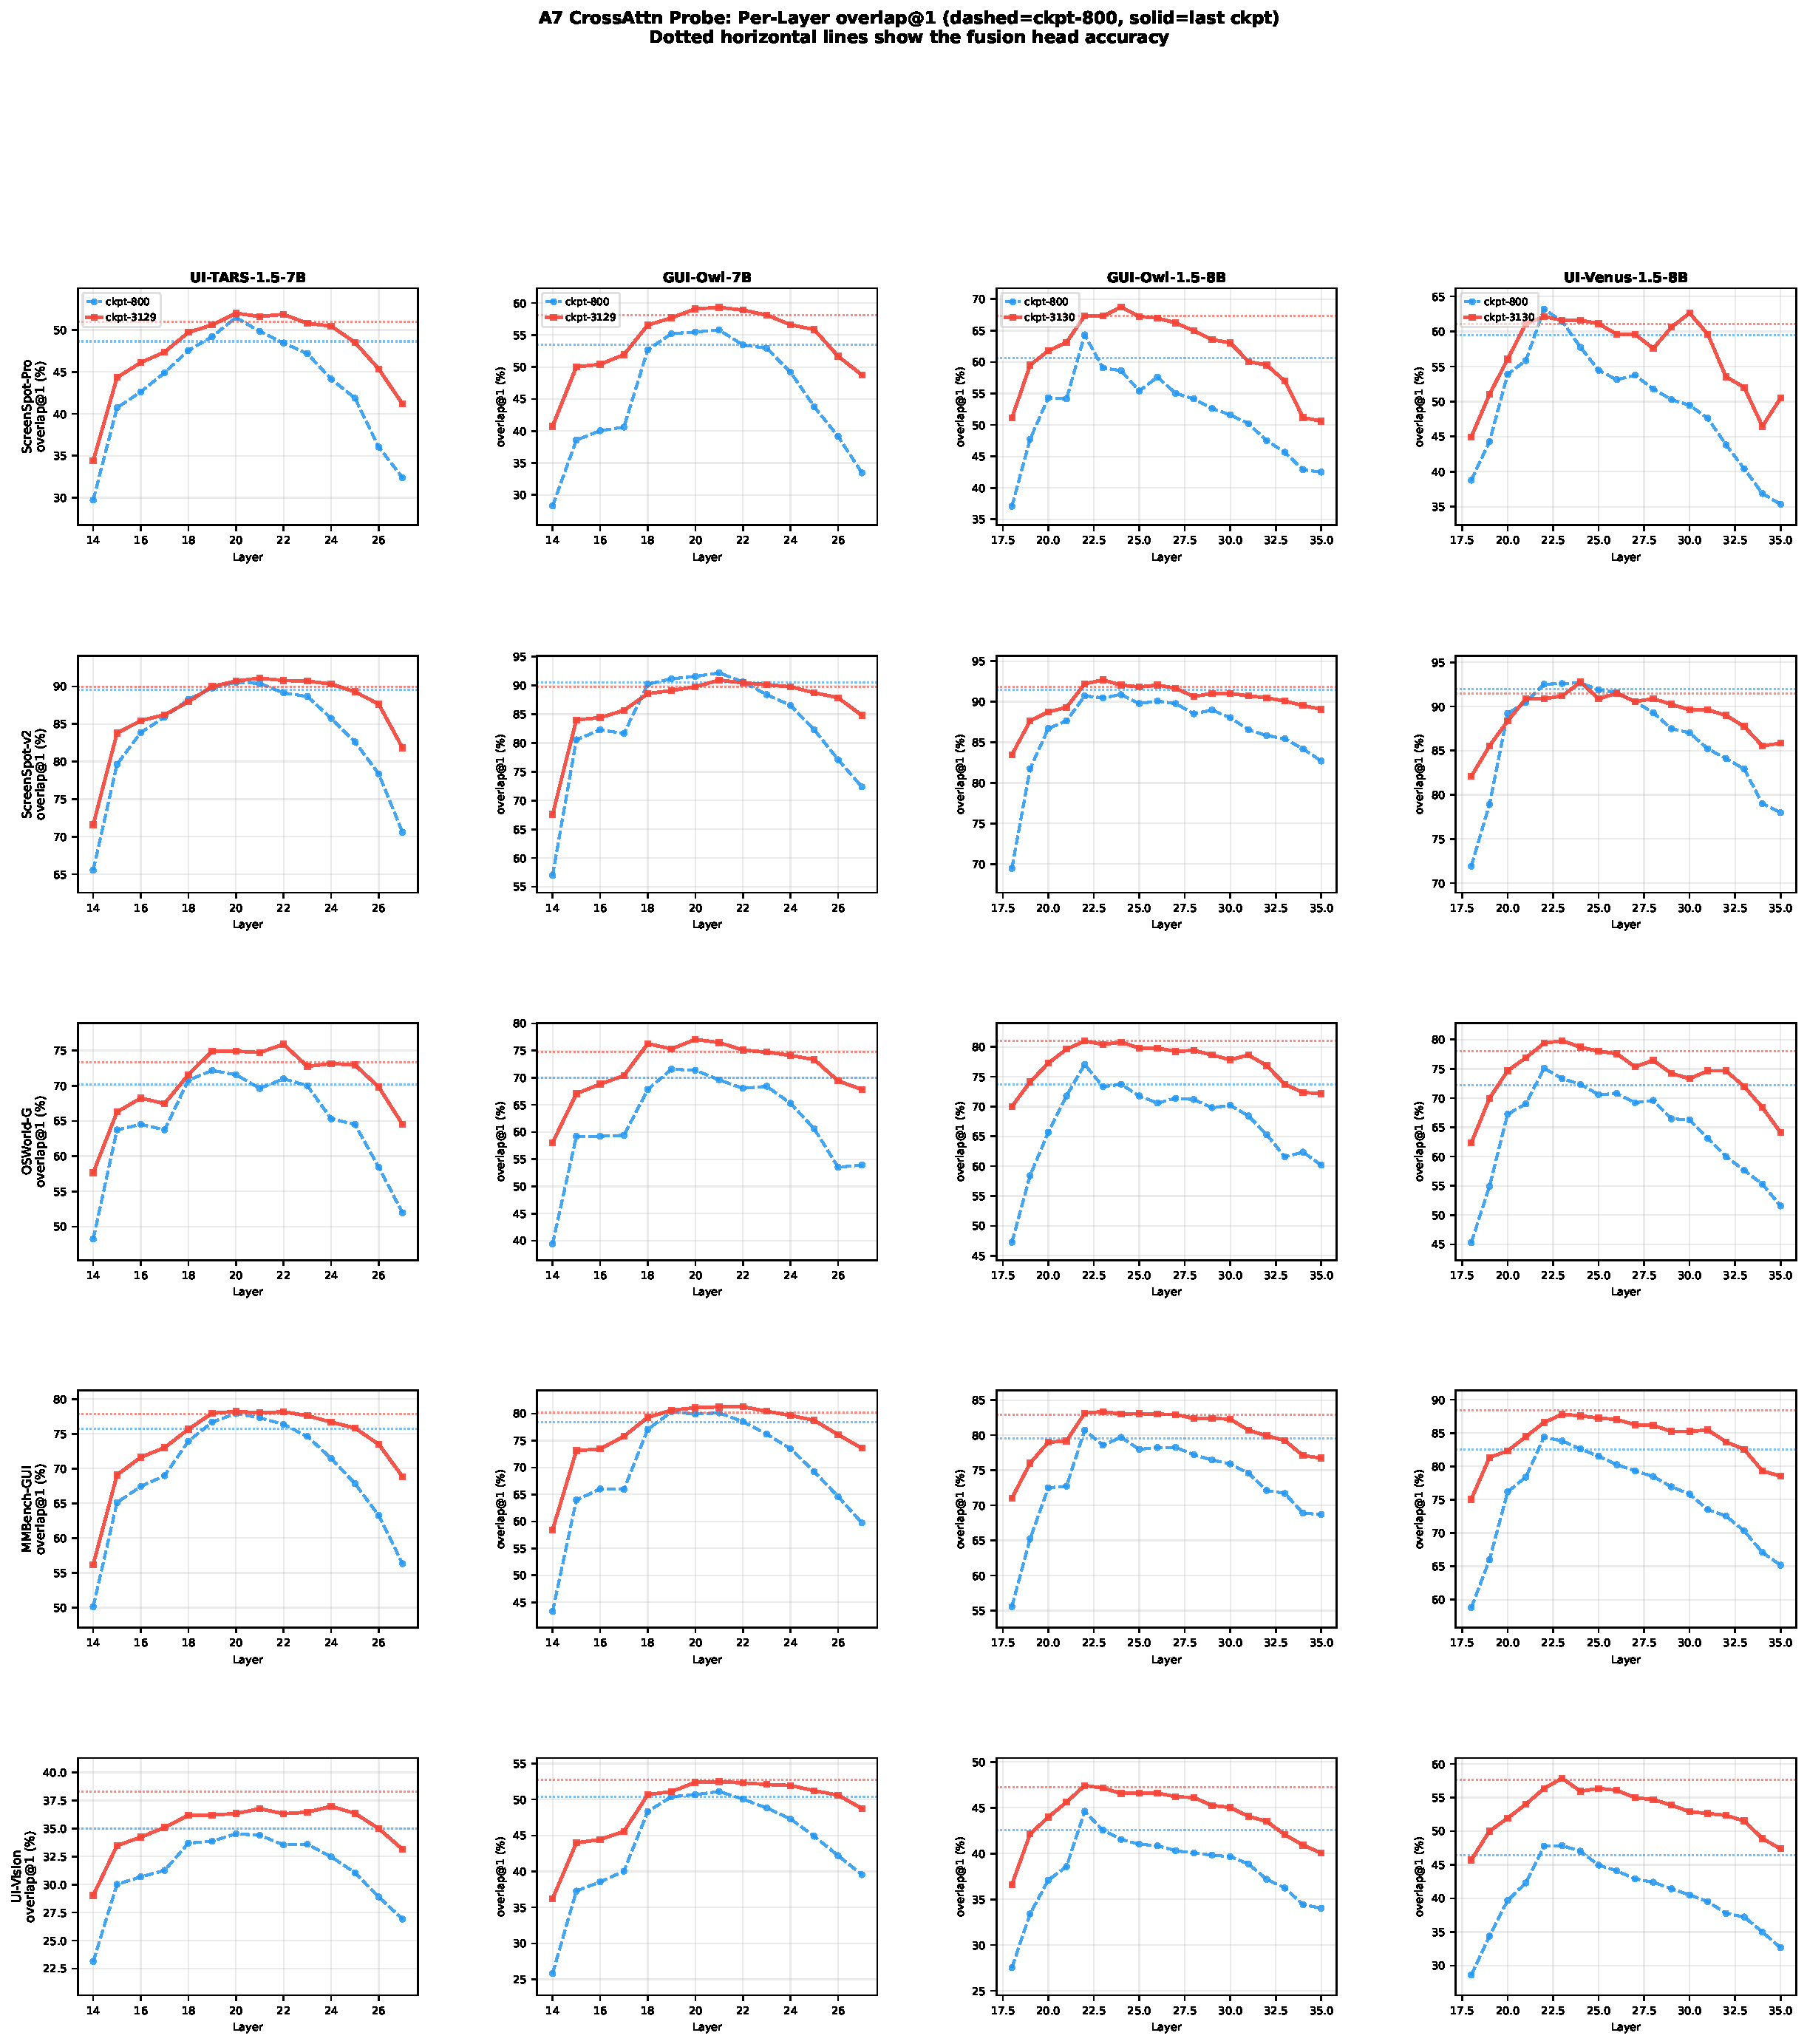
\includegraphics[width=\textwidth,
        height=0.80\textheight,]{figs/a7_layerwise_plots/a7_layerwise_combined.pdf}
  \caption{
    \textbf{Per-layer overlap@1 of A7 CrossAttn probes across all four backbone models and five benchmarks.}
    Each cell shows overlap@1 for a single probe layer evaluated independently (no cross-layer fusion).
    \textbf{Rows}: ScreenSpot-Pro (SS-Pro), ScreenSpot-v2 (SS-v2), OSWorld-G, MMBench-GUI, UI-Vision.
    \textbf{Columns}: UI-TARS-1.5-7B, GUI-Owl-7B, GUI-Owl-1.5-8B, UI-Venus-1.5-8B.
    \textbf{Blue dashed}: ckpt-800 (early training); \textbf{red solid}: last checkpoint (ckpt-3129 / ckpt-3130).
    \textbf{Horizontal dotted lines}: corresponding fusion head accuracy (the final \textsc{ZwerGe-UI} output).
    All four models exhibit an inverted-U spatial profile: accuracy peaks at intermediate layers and declines at the deepest layers, consistent with the coordinate serialization bottleneck (\S\ref{sec:analysis}).
    The fusion head (dotted) tracks the best single-layer probe within $1$--$3$\,pp across nearly all panels (and exceeds it on a few), providing a deployable, sample-adaptive readout that does not require per-benchmark layer selection.
  }
  \label{fig:app_perlayer_combined}
\end{figure*}

% ── Per-benchmark individual figures ─────────────────────────────────────────

Figures~\ref{fig:app_perlayer_sspro}--\ref{fig:app_perlayer_uivision} show the same data broken out by benchmark, at a larger scale for readability.

\begin{figure*}[p]
  \centering
  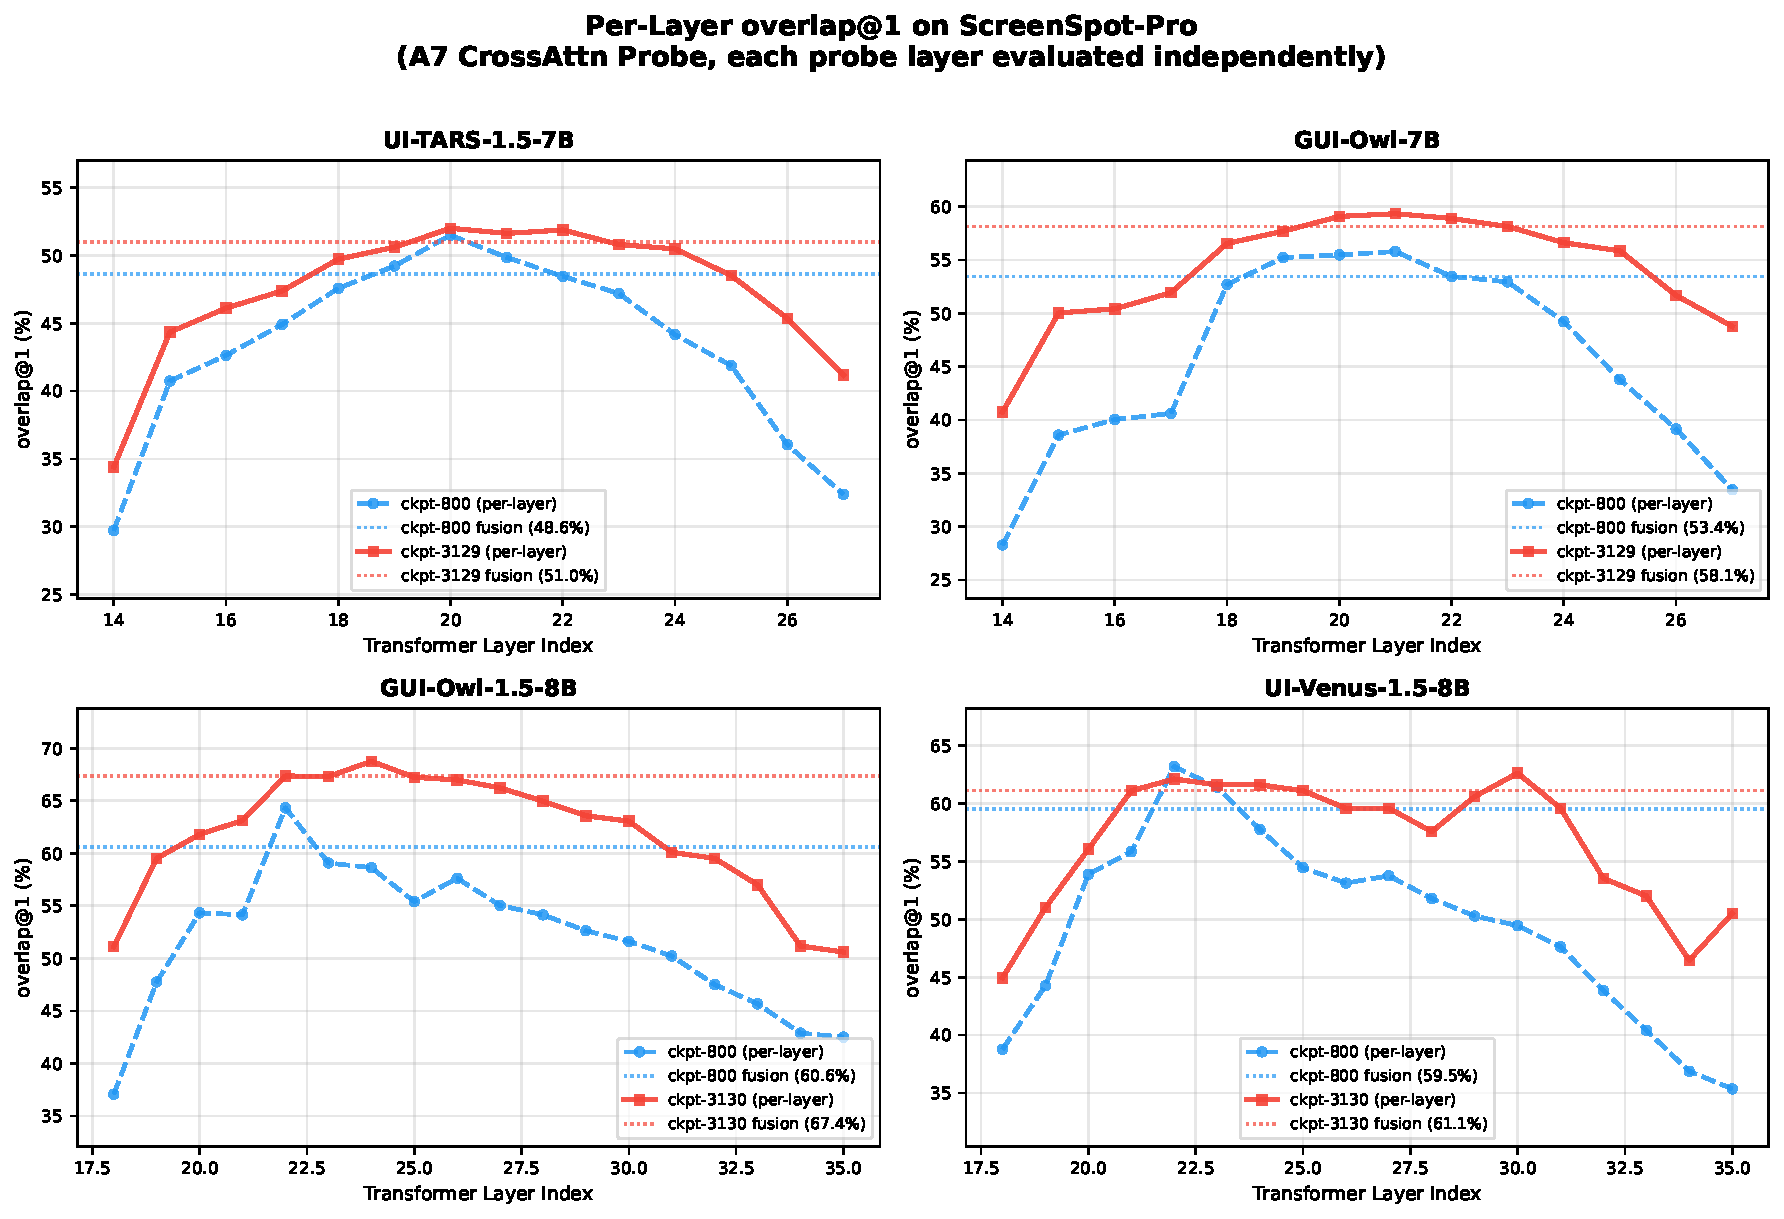
\includegraphics[width=0.92\textwidth]{figs/a7_layerwise_plots/a7_layerwise_ss_pro.pdf}
  \caption{
    \textbf{Per-layer overlap@1 on ScreenSpot-Pro.}
    ScreenSpot-Pro is the most demanding benchmark (fine-grained targets on high-resolution desktop screenshots).
    The inverted-U profile is the sharpest here, with the deepest layers showing the steepest decline,
    reflecting that high-resolution targets require the most precise spatial encoding and are most sensitive to the serialization shift in deep layers.
    Note that the vertical scales differ across panels to emphasize the shape of the curve within each model.
  }
  \label{fig:app_perlayer_sspro}
\end{figure*}

\begin{figure*}[p]
  \centering
  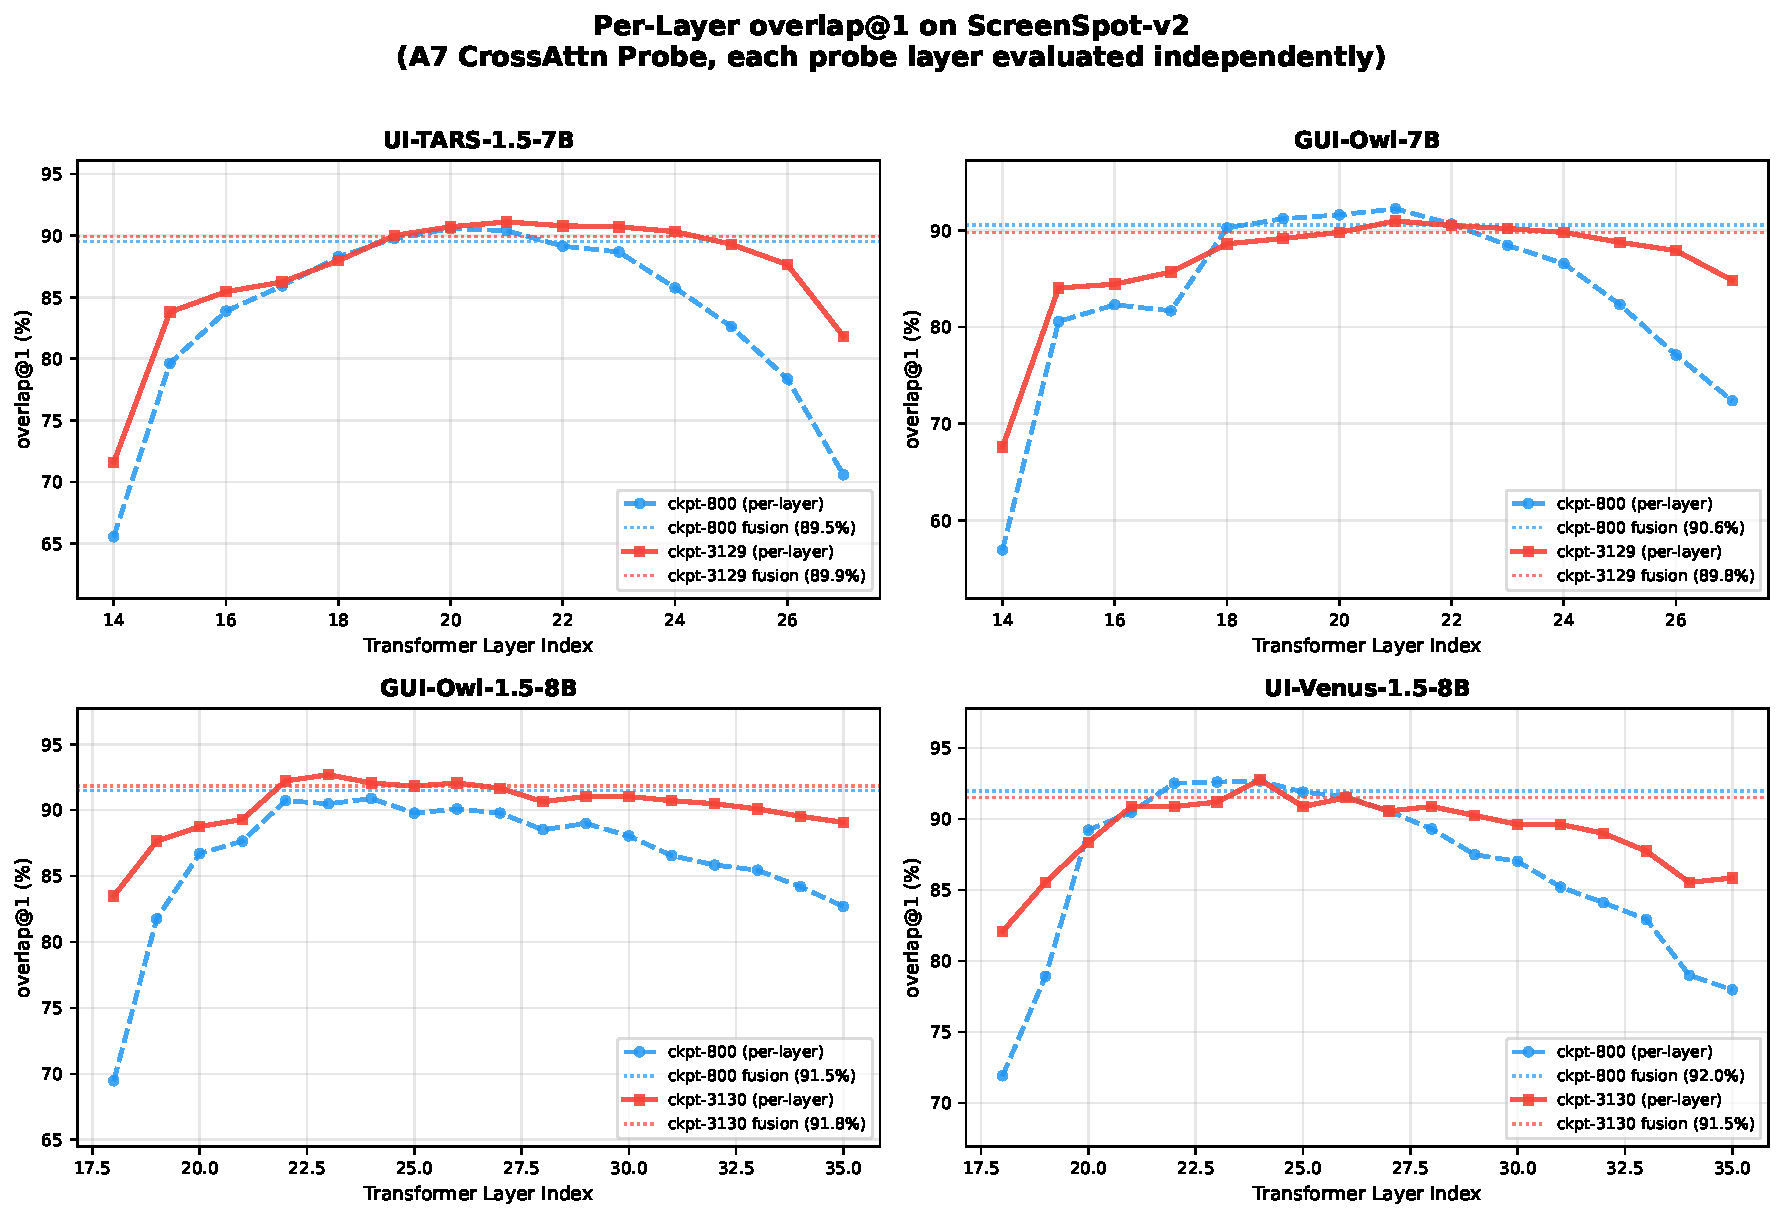
\includegraphics[width=0.92\textwidth]{figs/a7_layerwise_plots/a7_layerwise_ss_v2.pdf}
  \caption{
    \textbf{Per-layer overlap@1 on ScreenSpot-v2.}
    ScreenSpot-v2 is a moderate-resolution benchmark (mobile, desktop, web) where overall accuracy is already high ($>$87\% at ckpt-800).
    The inverted-U is shallower and the peak is broader compared to ScreenSpot-Pro,
    indicating that moderate-resolution grounding is less sensitive to which specific layer is read.
  }
  \label{fig:app_perlayer_ssv2}
\end{figure*}

\begin{figure*}[p]
  \centering
  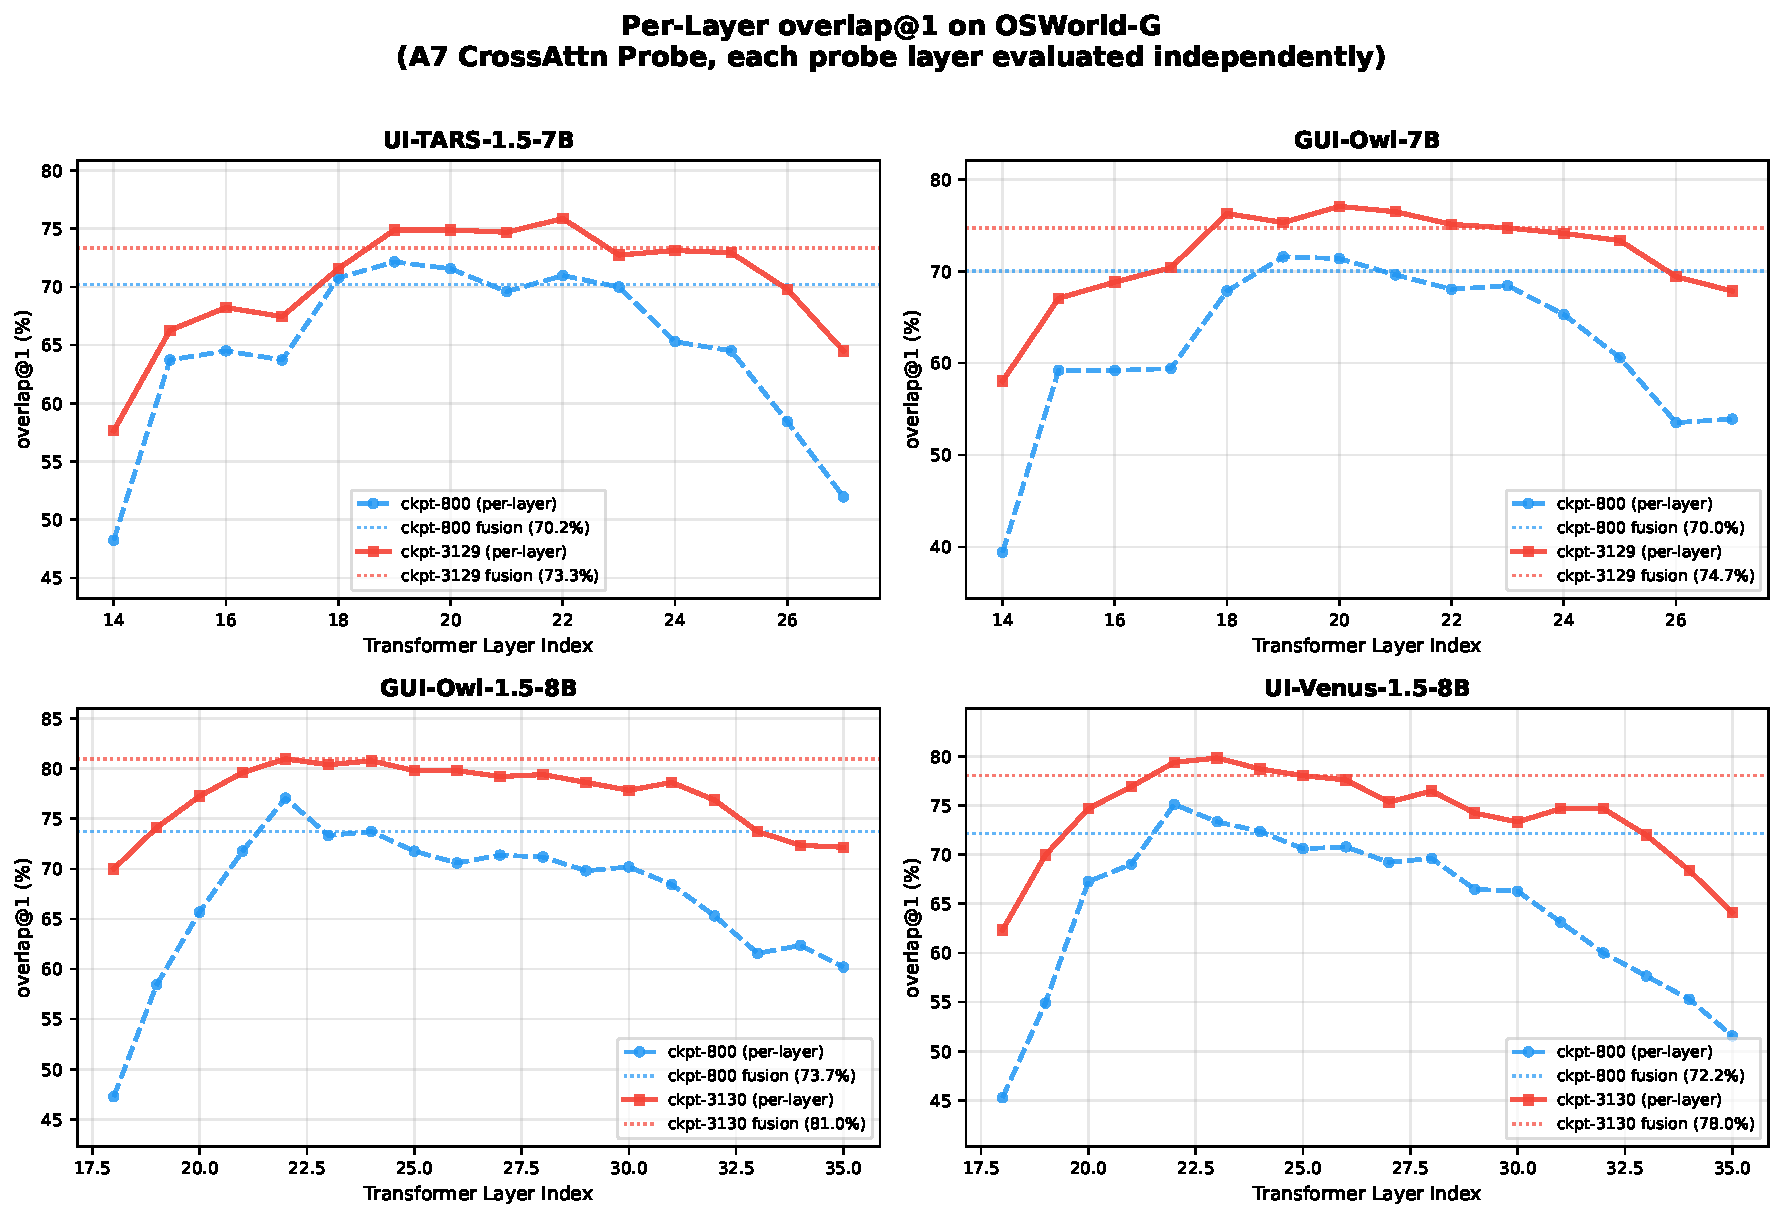
\includegraphics[width=0.92\textwidth]{figs/a7_layerwise_plots/a7_layerwise_osworld_g.pdf}
  \caption{
    \textbf{Per-layer overlap@1 on OSWorld-G.}
    OSWorld-G provides real computer-task GUI samples with diverse task types (Text Matching, Element Recognition, Layout Understanding, Fine-grained Manipulation).
    The per-layer profile shows a similar inverted-U shape but with a plateau over a wider middle range ($\sim$L18--L24 for 28-layer models),
    suggesting that layout-level spatial reasoning is distributed more broadly across intermediate layers than fine-grained element targeting.
  }
  \label{fig:app_perlayer_osworld}
\end{figure*}

\begin{figure*}[p]
  \centering
  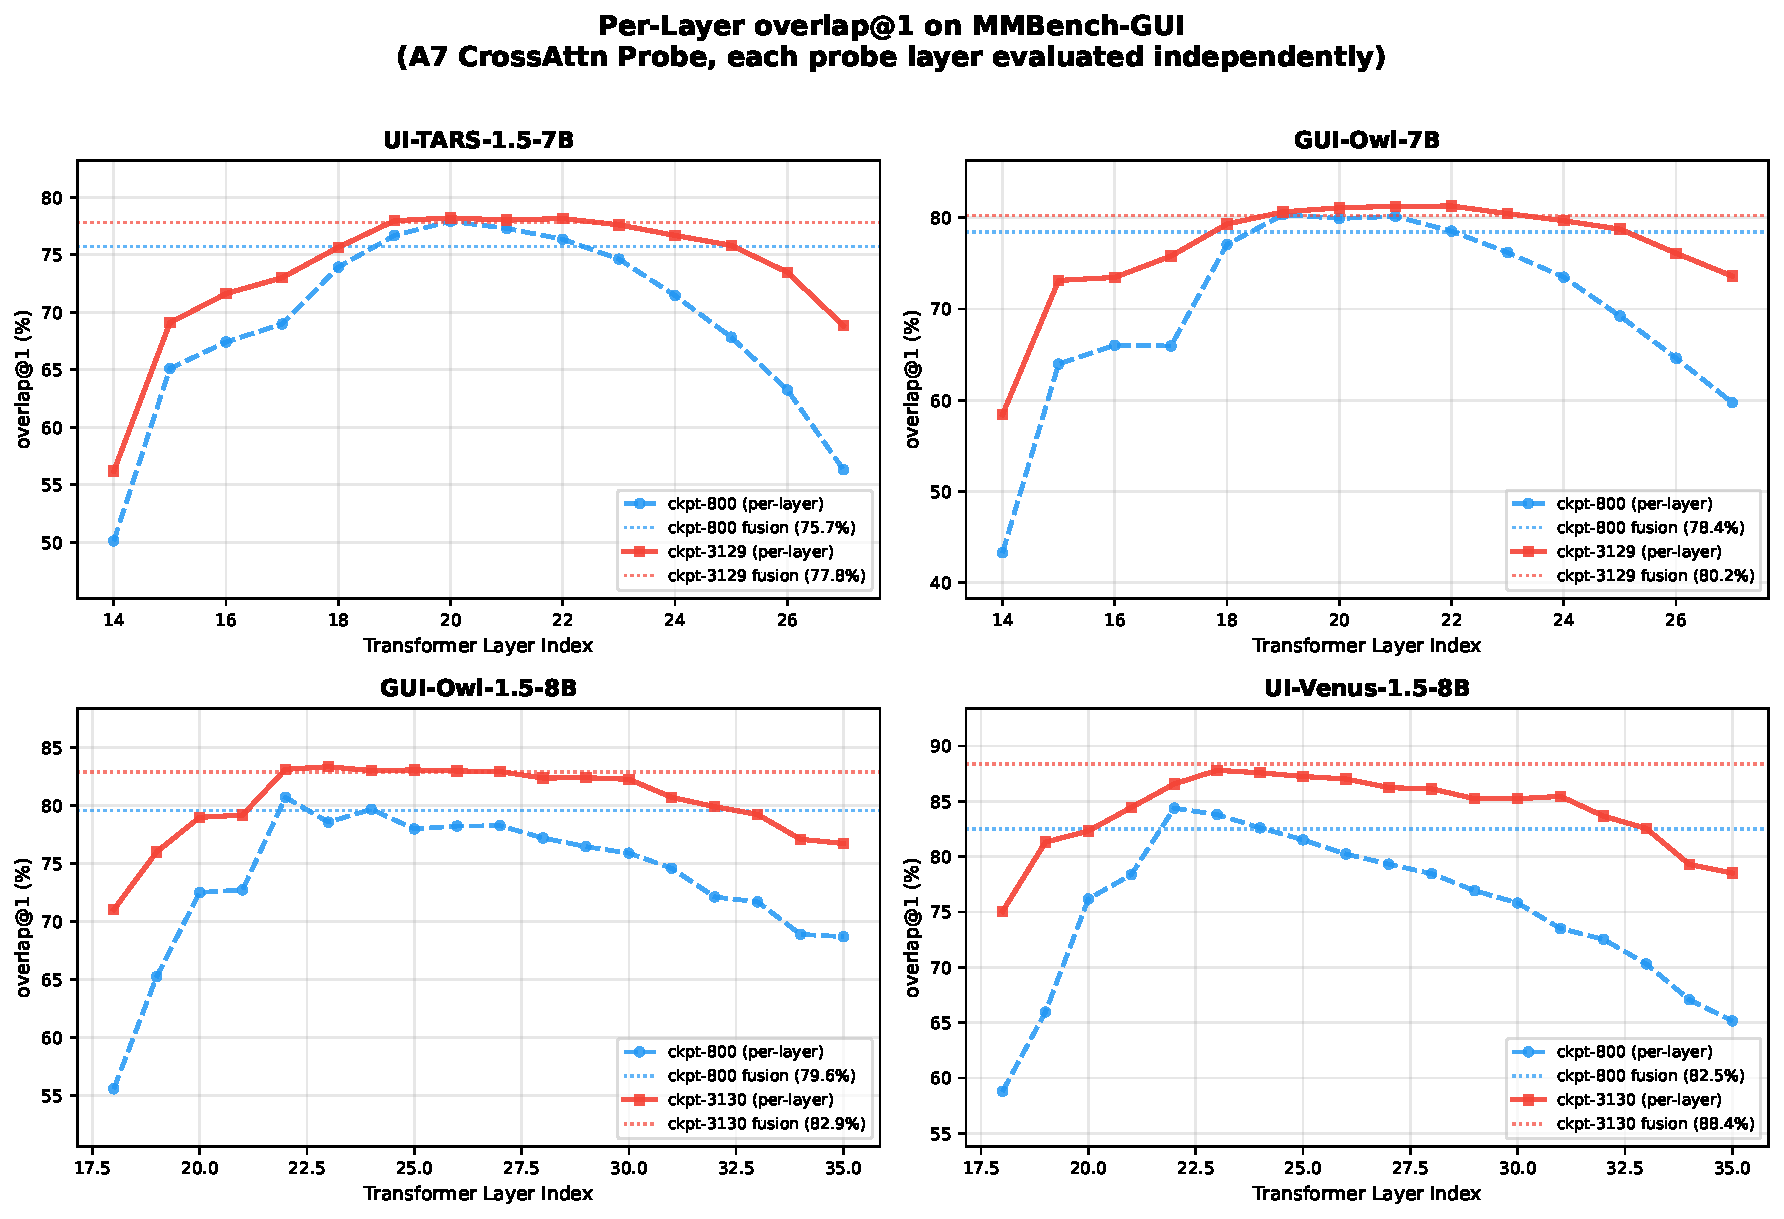
\includegraphics[width=0.92\textwidth]{figs/a7_layerwise_plots/a7_layerwise_mmbench.pdf}
  \caption{
    \textbf{Per-layer overlap@1 on MMBench-GUI.}
    MMBench-GUI covers six platforms (Windows, macOS, Linux, iOS, Android, Web).
    The per-layer curves are notably high even at ckpt-800 (blue dashed) for Qwen3-VL models (GUI-Owl-1.5-8B and UI-Venus-1.5-8B),
    reflecting that these models have strong cross-platform generalization already encoded in their intermediate representations.
    The gap between ckpt-800 and last checkpoint is smaller on MMBench-GUI than on ScreenSpot-Pro,
    suggesting that the per-layer signal saturates earlier on this benchmark.
  }
  \label{fig:app_perlayer_mmbench}
\end{figure*}

\begin{figure*}[p]
  \centering
  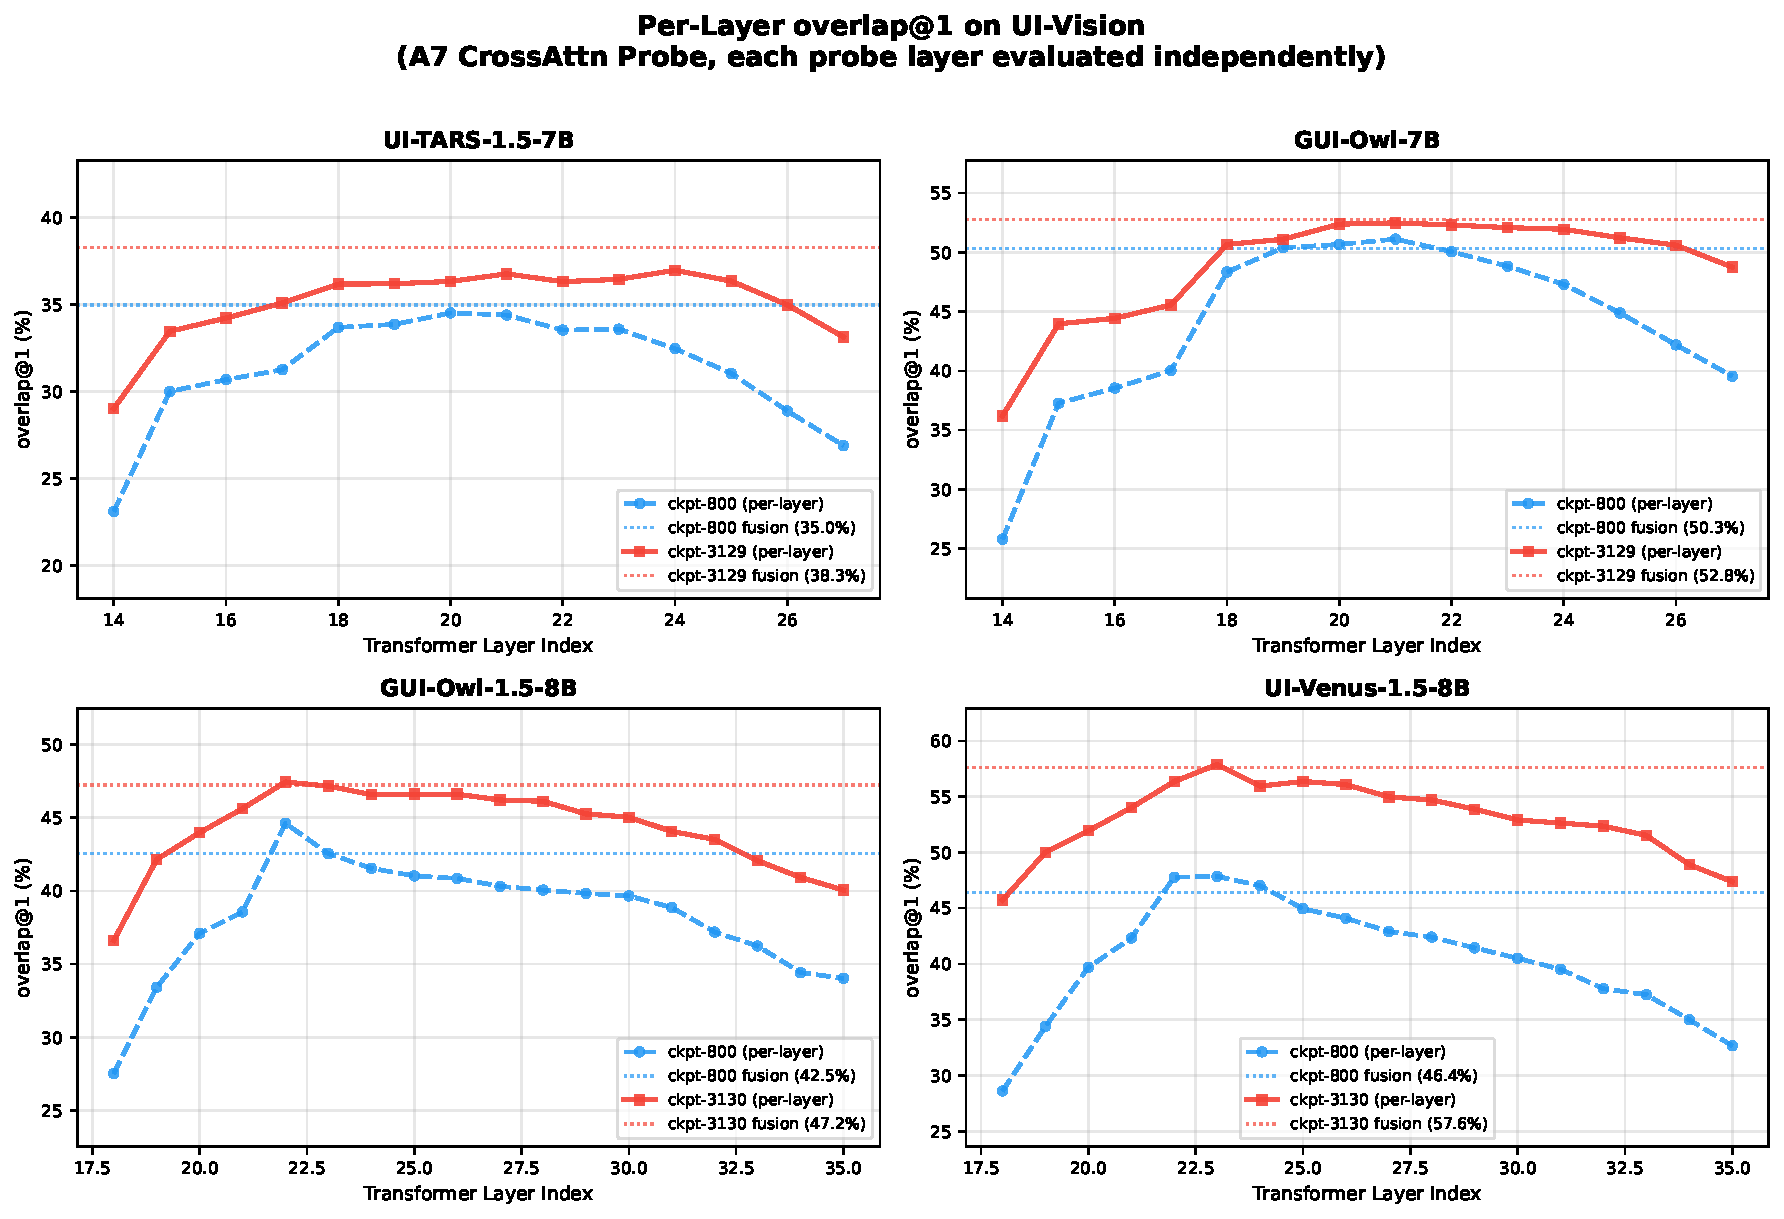
\includegraphics[width=0.92\textwidth]{figs/a7_layerwise_plots/a7_layerwise_ui_vision.pdf}
  \caption{
    \textbf{Per-layer overlap@1 on UI-Vision.}
    UI-Vision decomposes grounding into Basic, Functional, Spatial, and Layout subtypes; accuracy here represents the weighted average over all 5{,}790 samples.
    Per-layer accuracy is substantially lower on UI-Vision than on other benchmarks,
    particularly for Qwen2.5-VL models at early training (ckpt-800 for UI-TARS-1.5-7B peaks below 30\%),
    indicating that UI-Vision's diverse task composition is harder for intermediate probes to solve with limited training.
    The inverted-U is still present but shallower and shifted earlier (peak around L18--L20),
    possibly because UI-Vision includes layout-level tasks that require higher-level semantic understanding.
  }
  \label{fig:app_perlayer_uivision}
\end{figure*}


\label{sec:prompt}

\begin{figure*}[t]
\begin{tcolorbox}[colback=white, width=\linewidth, breakable, enhanced, 
                  title=Prompt for the UI-TARS-1.5 Model, fonttitle=\bfseries]

\lstset{
basicstyle=\scriptsize\ttfamily,
    columns=fullflexible,
    breaklines=true,
    breakatwhitespace=false,
    showstringspaces=false,
    lineskip=-1pt
}

\begin{lstlisting}
You are a helpful assistant.

You are a GUI agent. You are given a task and your action history, with screenshots.
You need to perform the next action to complete the task.

## Output Format
Action: ...

## Action Space
click(start_box='<|box_start|>(x1,y1)<|box_end|>')

## User Instruction
Task Instruction: {instruction}

\end{lstlisting}

\end{tcolorbox}
\end{figure*}
\begin{figure*}[t]
\begin{tcolorbox}[colback=white, width=\linewidth, breakable, enhanced, 
                  title=Prompt for the GUI-Owl Model, fonttitle=\bfseries, label=prompt:guiowl]

\lstset{
basicstyle=\scriptsize\ttfamily,
    columns=fullflexible,
    breaklines=true,
    breakatwhitespace=false,
    showstringspaces=false,
    lineskip=-1pt
}

\begin{lstlisting}
You are a helpful assistant.
# Tools
You may call one or more functions to assist with the user query.
You are provided with function signatures within <tools></tools> XML tags:
<tools>
{
    "type": "function",
    "function": {
        "name": "computer_use",
        "description": "Use a mouse to interact with a computer screen."
                    "* The screen's resolution is ${height}x${width}."
                    "* Make sure to click any buttons, links, icons, etc with the cursor tip in the center of the element. Don't click boxes on their edges unless asked.",
        "parameters": {
            "properties": {
                "action": {
                    "description": "The action to perform. The available actions are:"
                                "* `left_click`: Click the left mouse button at a specified (x, y) pixel coordinate on the screen.",
                    "enum": ["left_click"],
                    "type": "string"
                },
                "coordinate": {
                    "description": "(x, y): The x (pixels from the left edge) and y (pixels from the top edge) coordinates to click.",
                    "type": "array"
                }
            },
            "required": ["action"],
            "type": "object"
        }
    }
}
</tools>
For each function call, return a json object with function name and arguments within <tool_call></tool_call> XML tags:
<tool_call>
{"name": <function-name>, "arguments": <args-json-object>}
</tool_call>

## User Instruction
Please complete the following tasks by clicking using `left_click` function: {instruction}

\end{lstlisting}

\end{tcolorbox}
\end{figure*}
\begin{figure*}[t]
\begin{tcolorbox}[colback=white, width=\linewidth, breakable, enhanced, 
                  title=Prompt for the GUI-Owl-1.5 Model, fonttitle=\bfseries]

\lstset{
basicstyle=\scriptsize\ttfamily,
    columns=fullflexible,
    breaklines=true,
    breakatwhitespace=false,
    showstringspaces=false,
    lineskip=-1pt
}

\begin{lstlisting}
# Tools

You may call one or more functions to assist with the user query.

You are provided with function signatures within <tools></tools> XML tags:
<tools>
{"type": "function", "function": {"name": "computer_use", "description": "Use a mouse to interact with a computer.\n* The screen's resolution is 1000x1000.\n* Make sure to click any buttons, links, icons, etc with the cursor tip in the center of the element. Don't click boxes on their edges unless asked.", "parameters": {"properties": {"action": {"description": "The action to perform. The available actions are:\n* `left_click`: Click the left mouse button with coordinate (x, y) pixel coordinate on the screen.", "enum": ["left_click"], "type": "string"}, "coordinate": {"description": "(x, y): The x (pixels from the left edge) and y (pixels from the top edge) coordinates to click.", "type": "array"}}, "required": ["action"], "type": "object"}}}
</tools>

For each function call, return a json object with function name and arguments within <tool_call></tool_call> XML tags:
<tool_call>
{"name": <function-name>, "arguments": <args-json-object>}
</tool_call>

## User Instruction
{instruction}

\end{lstlisting}

\end{tcolorbox}
\end{figure*}
\begin{figure*}[t]
\begin{tcolorbox}[colback=white, width=\linewidth, breakable, enhanced, 
                  title=Prompt for the UI-Venus-1.5 Model, fonttitle=\bfseries, label=prompt:uivenus15]
\lstset{
basicstyle=\scriptsize\ttfamily,
    columns=fullflexible,
    breaklines=true,
    breakatwhitespace=false,
    showstringspaces=false,
    lineskip=-1pt
}

\begin{lstlisting}
Output the center point of the position corresponding to the following instruction: {instruction}.

The output should just be the coordinates of a point, in the format [x,y].

\end{lstlisting}

\end{tcolorbox}
\end{figure*}

\begin{figure*}[t]
\begin{tcolorbox}[colback=white, width=\linewidth, breakable, enhanced, 
                  title=Prompt for the UI-TARS-1.5 Retrofit Model, fonttitle=\bfseries]

\lstset{
basicstyle=\scriptsize\ttfamily,
    columns=fullflexible,
    breaklines=true,
    breakatwhitespace=false,
    showstringspaces=false,
    lineskip=-1pt
}

\begin{lstlisting}
[System]
You are a GUI agent. You are given a task and a screenshot.
You need to perform the next action to complete the task.

## Output Format

Action: ...

## Action Space

click(start_box='<|ground|><|pointer_start|><|pointer_pad|><|pointer_end|>')

[User]
<image>
{instruction}

[Assistant]
click(start_box='<|ground|><|pointer_start|><|pointer_pad|><|pointer_end|>')
\end{lstlisting}

\end{tcolorbox}
\end{figure*}
\begin{figure*}[t]
\begin{tcolorbox}[colback=white, width=\linewidth, breakable, enhanced, 
                  title=Prompt for the GUI-Owl-7B / GUI-Owl-1.5 Retrofit Model, fonttitle=\bfseries, label=prompt:guiowl-retrofit]
\lstset{
basicstyle=\scriptsize\ttfamily,
    columns=fullflexible,
    breaklines=true,
    breakatwhitespace=false,
    showstringspaces=false,
    lineskip=-1pt
}

\begin{lstlisting}
[System]
# Tools

You may call one or more functions to assist with the user query.

You are provided with function signatures within <tools></tools> XML tags:
<tools>
{"type": "function", "function": {
"name": "computer_use",
"description": "Use a mouse and keyboard to interact with a computer, and take screenshots. This is an interface to a desktop GUI. You do not have access to a terminal or applications menu. You must click on desktop icons to start applications. * The screen's resolution is 1000x1000.\n* Make sure to click buttons, links, icons, etc with the cursor tip in the center of the element. Don't click boxes on their edges unless asked.",
"parameters": {"properties": {"action": {"description": "The action to perform. The available actions are:\n* `left_click`: Click the left mouse button at coordinate (x, y) pixel coordinate on the screen.", "enum": ["left_click"], "type": "string"}, "coordinate": {"description": "(x, y): The x (pixels from the left edge) and y (pixels from the top edge) coordinates to click. Required only by `action=left_click`.", "type": "array"}}, "required": ["action", "coordinate"], "type": "object"}}}
</tools>

For each function call, return a json object with function name and arguments within <tool_call></tool_call> XML tags:
<tool_call>
{"name": "computer_use", "arguments": {"action": "left_click", "coordinate": [<|ground|><|pointer_start|><|pointer_pad|><|pointer_end|>]}}
</tool_call>

[User]
<image>
{instruction}

[Assistant]
<tool_call>
{"name": "computer_use", "arguments": {"action": "left_click", "coordinate": [<|ground|><|pointer_start|><|pointer_pad|><|pointer_end|>]}}
</tool_call>
\end{lstlisting}

\end{tcolorbox}
\end{figure*}
\begin{figure*}[t]
\begin{tcolorbox}[colback=white, width=\linewidth, breakable, enhanced, 
                  title=Prompt for the UI-Venus-1.5 Retrofit Model, fonttitle=\bfseries, label=prompt:uivenus-retrofit]

\lstset{
basicstyle=\scriptsize\ttfamily,
    columns=fullflexible,
    breaklines=true,
    breakatwhitespace=false,
    showstringspaces=false,
    lineskip=-1pt
}

\begin{lstlisting}
[User]
<image>
Output the center point of the position corresponding to the following instruction:
{instruction}.

The output should just be the coordinates of a point, in the format
[<|ground|><|pointer_start|><|pointer_pad|><|pointer_end|>].

[Assistant]
[<|ground|><|pointer_start|><|pointer_pad|><|pointer_end|>]
\end{lstlisting}

\end{tcolorbox}
\end{figure*}



\label{sec:vis1}

\begin{figure*}[t]
    \centering
    \begin{subfigure}{0.75\textwidth}
        \centering
        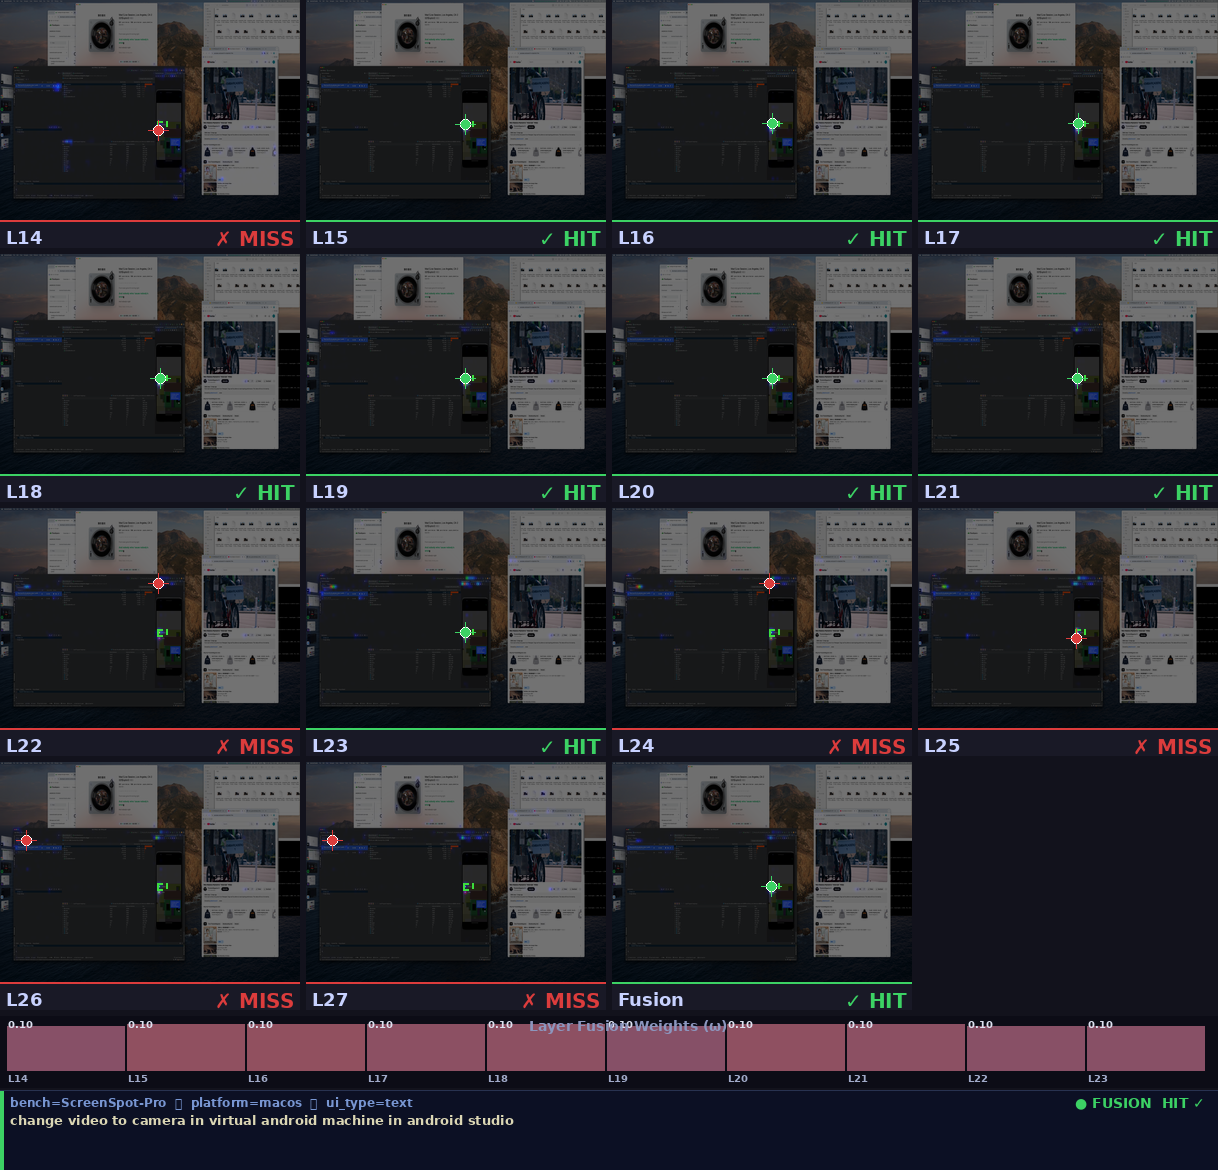
\includegraphics[width=\linewidth]{figs/append/uitars/idx00021.png}
    \end{subfigure}

    \vspace{0.6em}

    \begin{subfigure}{0.75\textwidth}
        \centering
        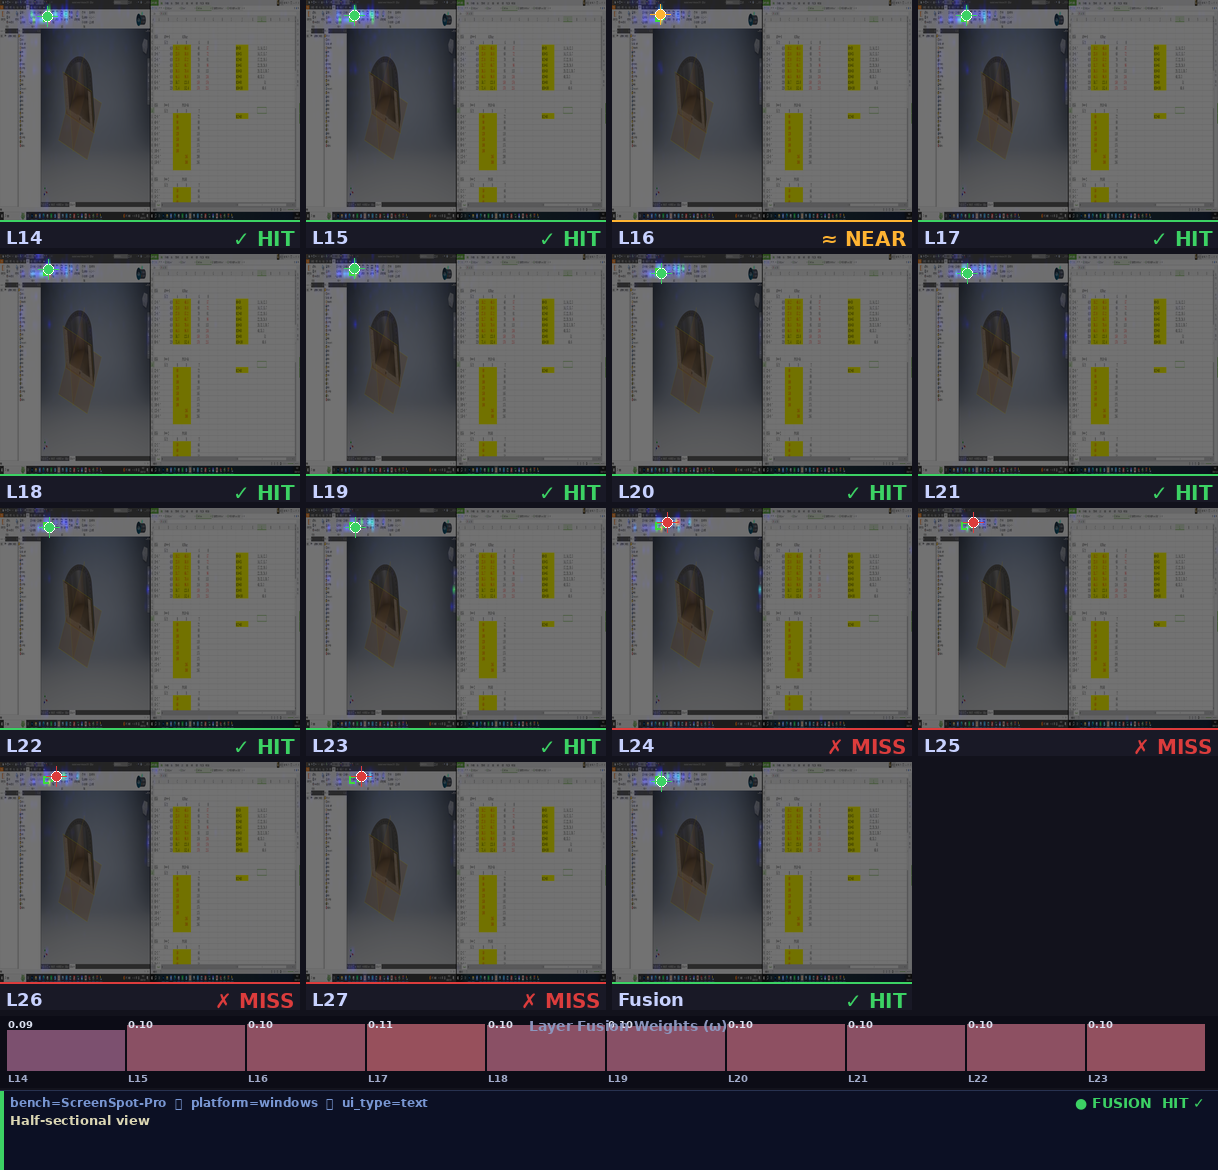
\includegraphics[width=\linewidth]{figs/append/uitars/idx00440.png}
    \end{subfigure}

    \caption{Successful cases of UI-TARS-1.5-7B on ScreenSpot-Pro}
    \label{fig:uitars15_screenspotpro_success}
\end{figure*}


\begin{figure*}[t]
    \centering
    \begin{subfigure}{0.75\textwidth}
        \centering
        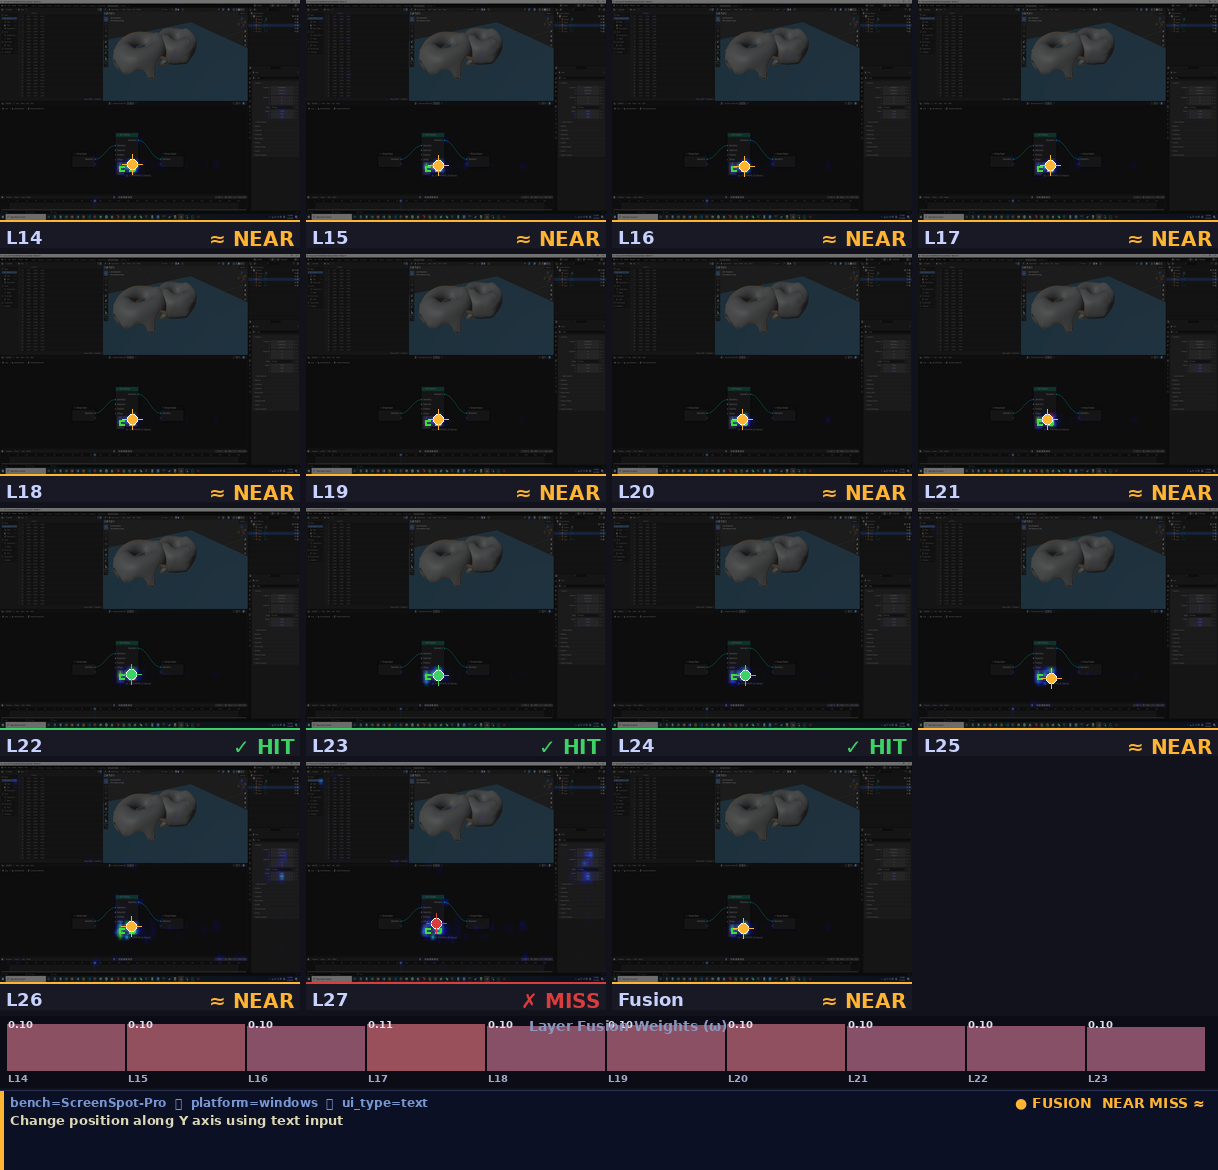
\includegraphics[width=\linewidth]{figs/append/uitars/idx00114.png}
    \end{subfigure}

    \vspace{0.6em}

    \begin{subfigure}{0.75\textwidth}
        \centering
        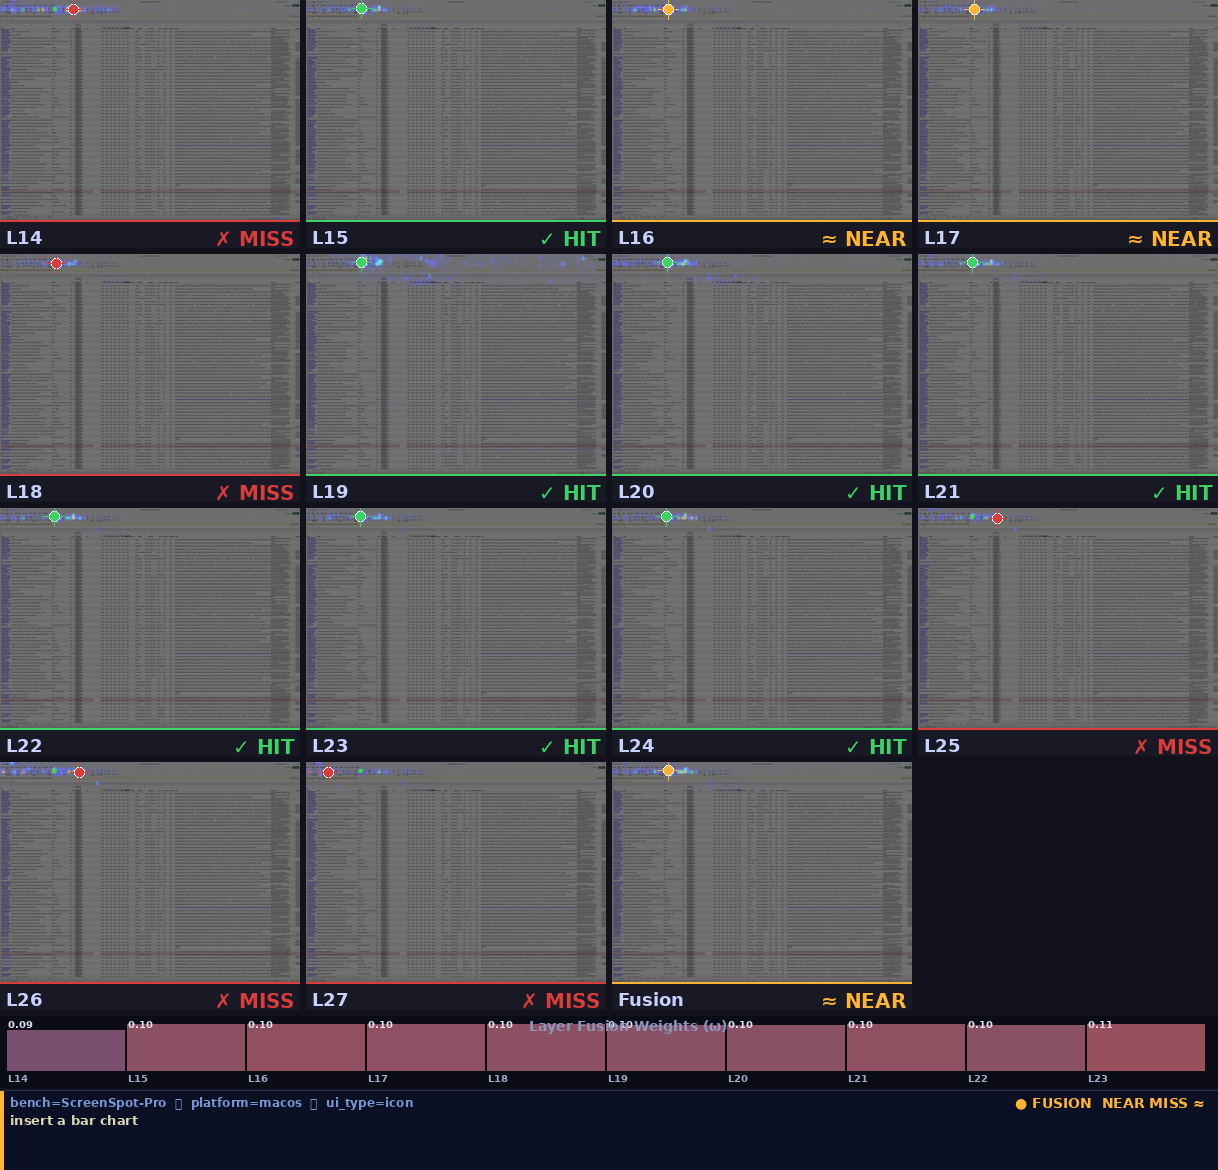
\includegraphics[width=\linewidth]{figs/append/uitars/idx00329.png}
    \end{subfigure}

    \caption{Failure cases of UI-TARS-1.5-7B on ScreenSpot-Pro}
    \label{fig:uitars15_screenspotpro_success}
\end{figure*}


\label{sec:vis}

\begin{figure*}[t]
    \centering
    \begin{subfigure}{0.65\textwidth}
        \centering
        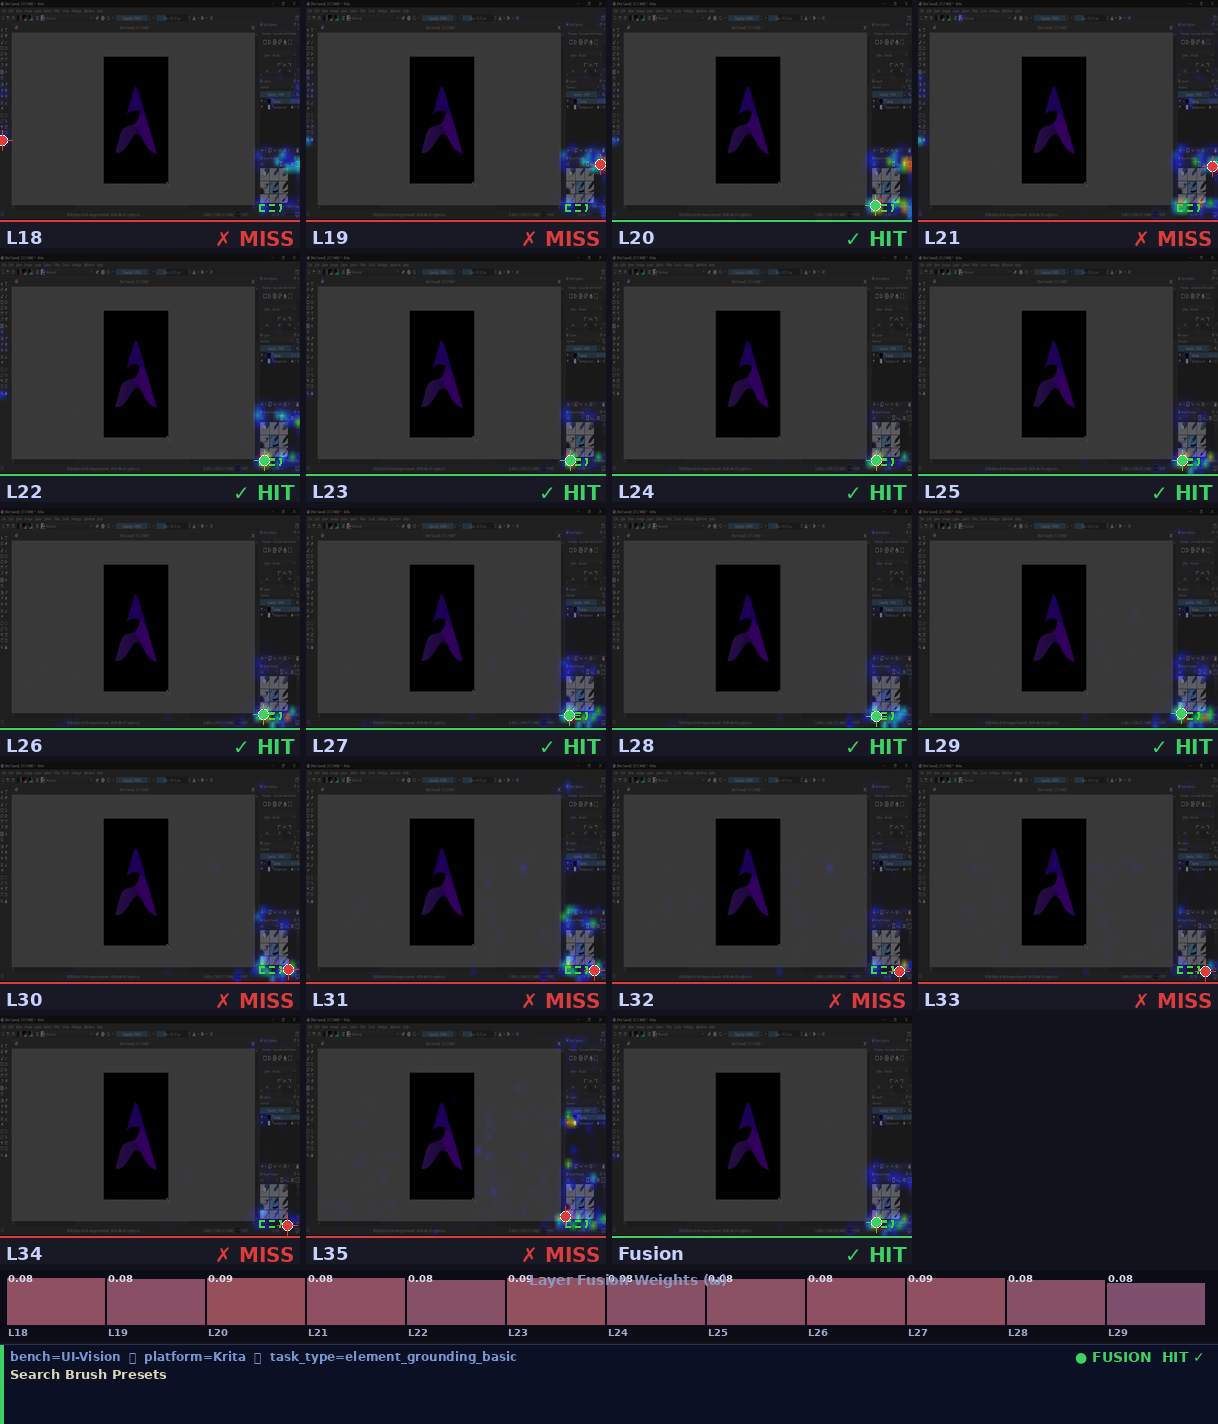
\includegraphics[width=\linewidth]{figs/append/uivenus/idx00015.png}
    \end{subfigure}

    \vspace{0.6em}

    \begin{subfigure}{0.65\textwidth}
        \centering
        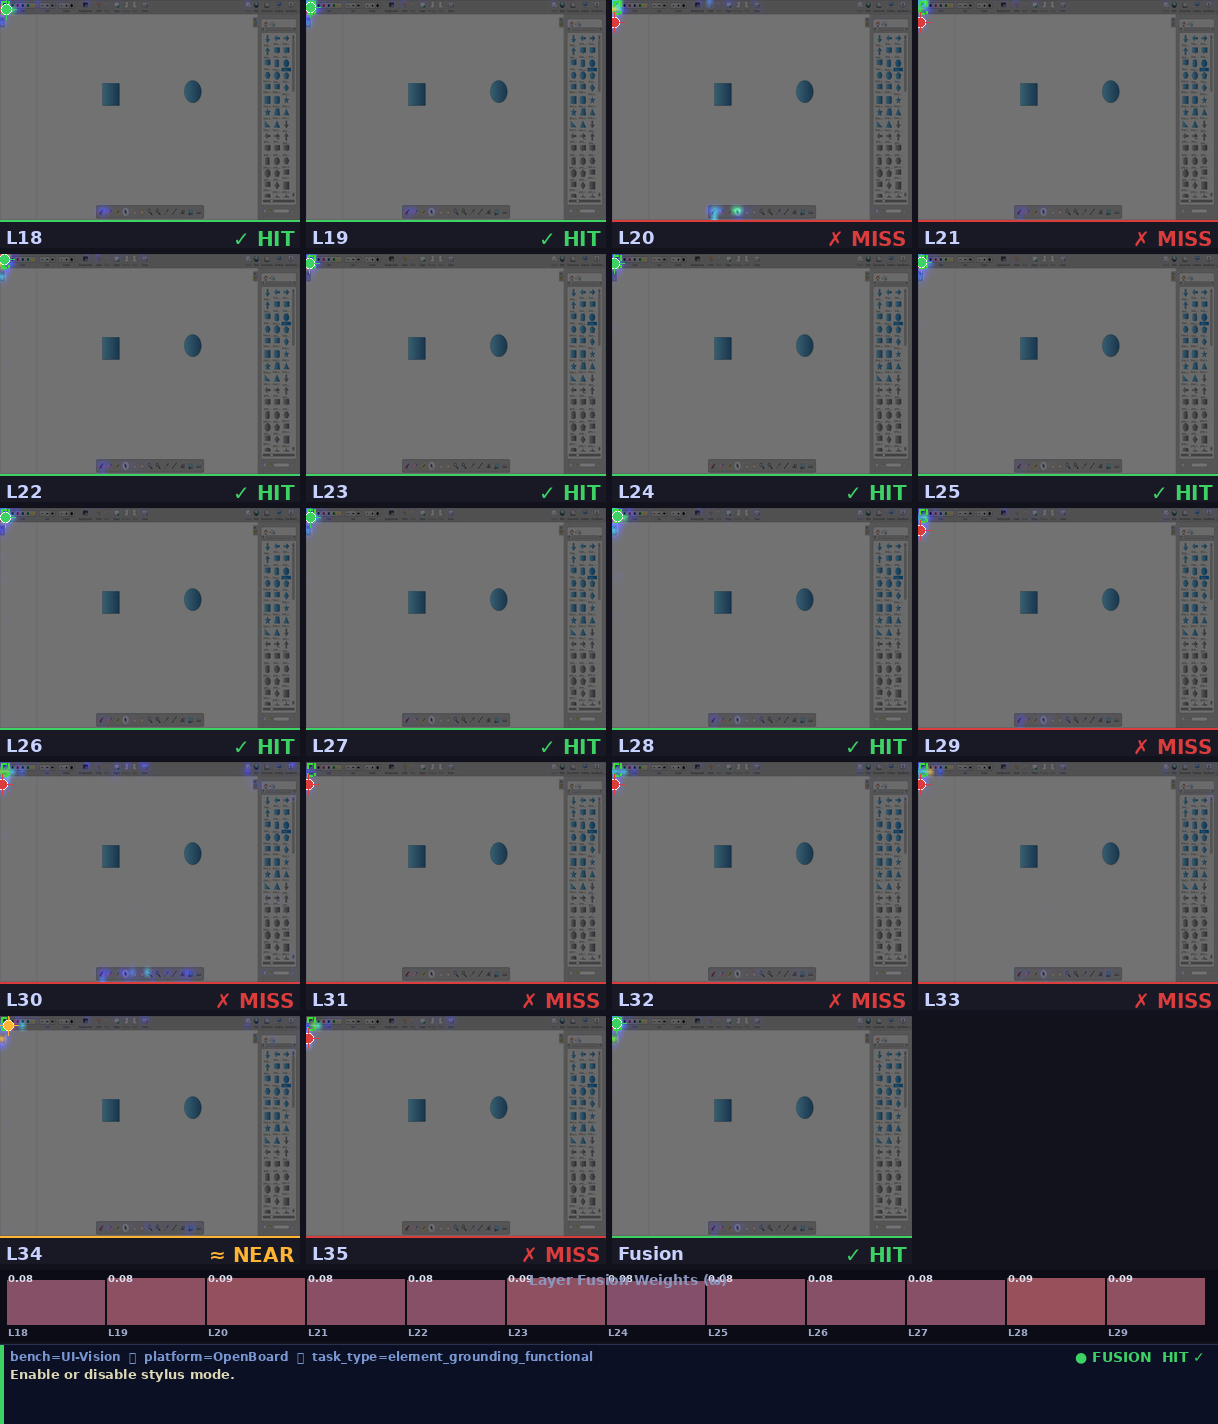
\includegraphics[width=\linewidth]{figs/append/uivenus/idx02155.png}
    \end{subfigure}

    \caption{Successful cases of UI-Venus-1.5-8B on MMBench-GUI-L2}
    \label{fig:uitars15_screenspotpro_success}
\end{figure*}


\begin{figure*}[t]
    \centering
    \begin{subfigure}{0.65\textwidth}
        \centering
        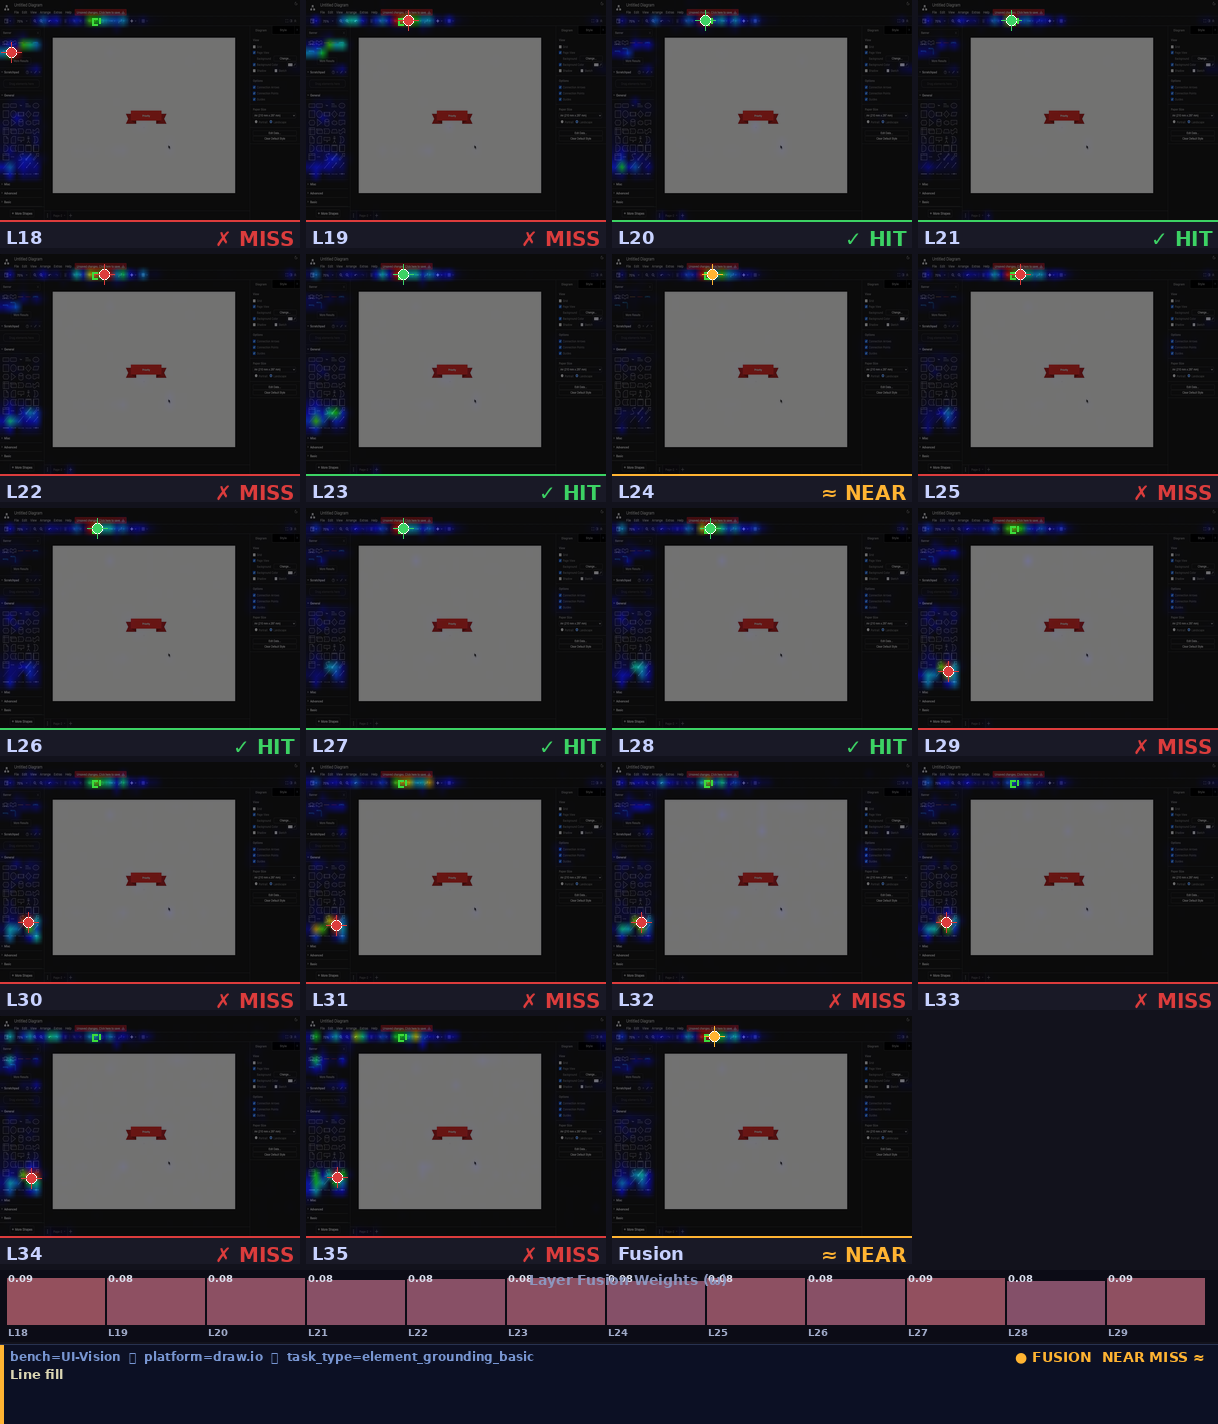
\includegraphics[width=\linewidth]{figs/append/uivenus/idx00405.png}
    \end{subfigure}

    \vspace{0.6em}

    \begin{subfigure}{0.65\textwidth}
        \centering
        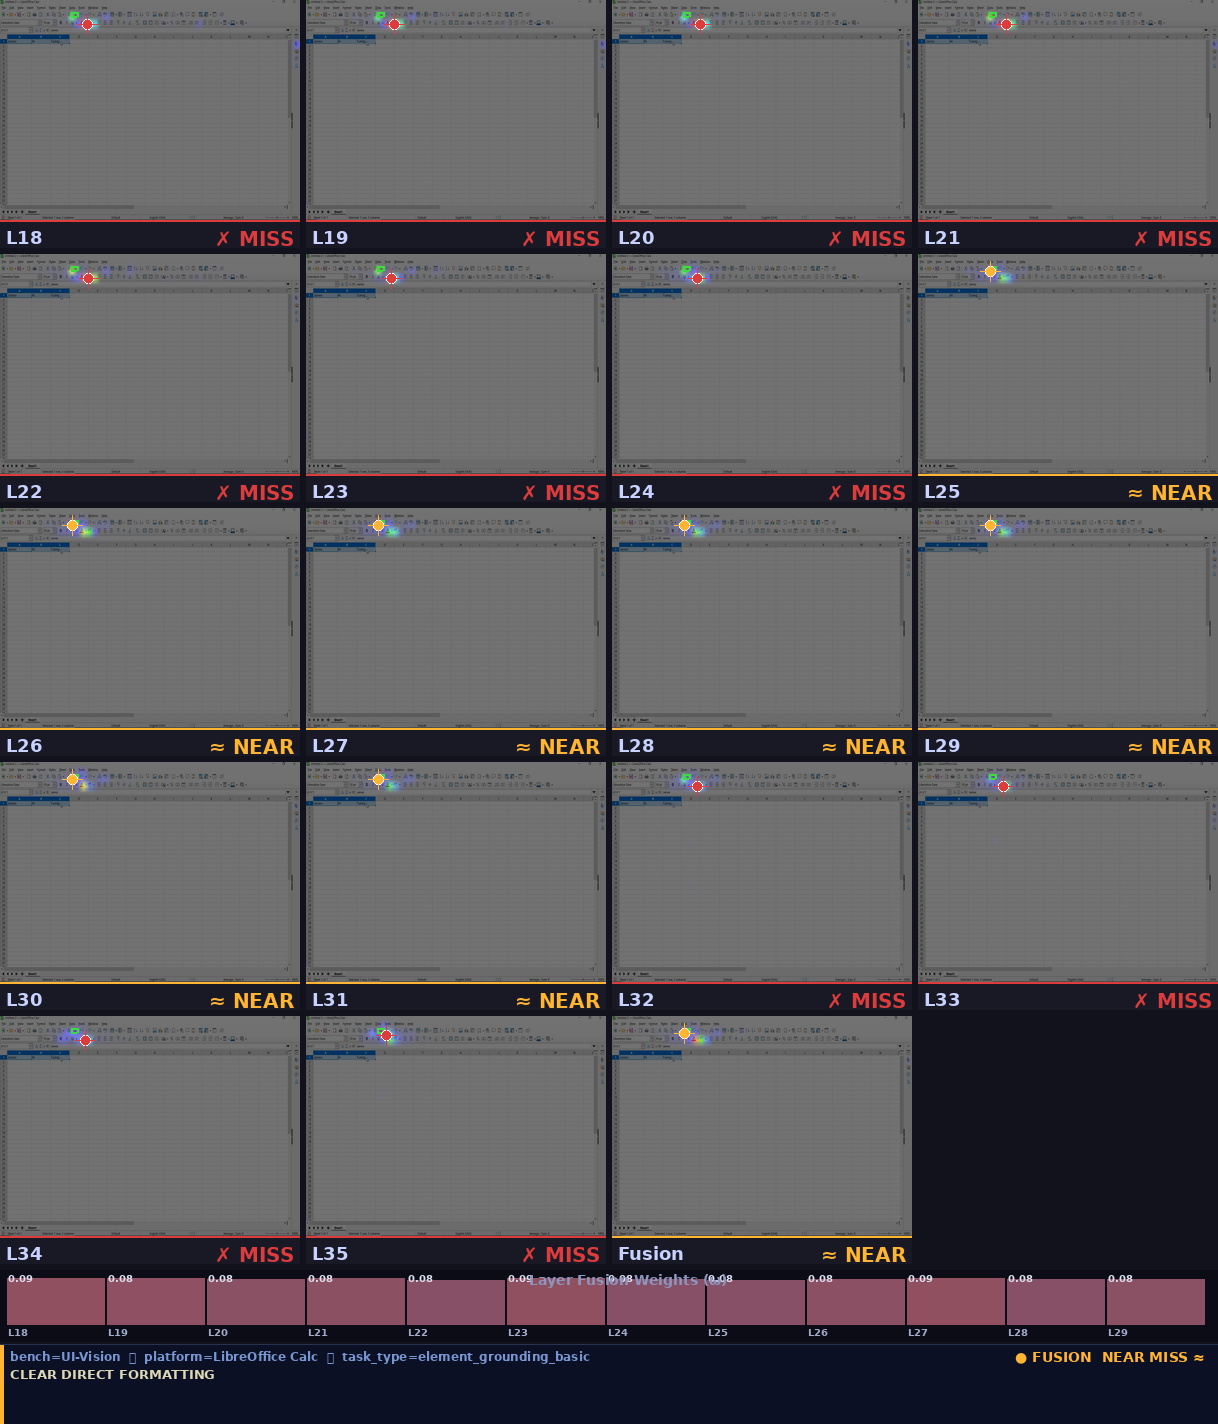
\includegraphics[width=\linewidth]{figs/append/uivenus/idx00493.png}
    \end{subfigure}

    \caption{Failure cases of UI-Venus-1.5-8B on MMBench-GUI-L2}
    \label{fig:uitars15_screenspotpro_success}
\end{figure*}

% ==============================================================================
% Appendix: Robustness, Controls, and Statistical Stability
% ==============================================================================

\section{Robustness, Controls, and Statistical Stability}
\label{app:controls}

This appendix consolidates the controls and uncertainty quantification requested
by the reviewers, all computed on the A8 (checkpoint-2800) probes used in the main
text. All scripts and raw JSON are released with the submission.

\paragraph{OOD layout generalization (4KeN-W4, eKpD-W2).}
Table~\ref{tab:ood_peak_layer} reports the spatial-peak layer $L^*$ for each
(model, benchmark) cell. $L^*$ varies by at most $3$ layers within each model
across the five benchmarks (std $\le 1.1$), including the distribution-shifted
UI-Vision and MMBench-GUI. The inverted-U (peak $>$ final) holds in $20/20$ cells.
\begin{table}[t]
\centering\small
\setlength{\tabcolsep}{4pt}
\begin{tabular}{lcccccccc}
\toprule
& SS-Pro & SS-v2 & OSWorld-G & UI-Vision & MMBench-GUI & mean & std & range$\downarrow$\\
\midrule
UI-TARS-1.5-7B & 20 & 21 & 21 & 23 & 20 & 21.0 & 1.10 & 3\\
GUI-Owl-7B & 19 & 21 & 20 & 20 & 20 & 20.0 & 0.63 & 2\\
GUI-Owl-1.5-8B-Instruct & 24 & 23 & 23 & 22 & 25 & 23.4 & 1.02 & 3\\
UI-Venus-1.5-8B & 23 & 25 & 25 & 24 & 24 & 24.2 & 0.75 & 2\\
\bottomrule
\end{tabular}
\caption{\textbf{Spatial-peak layer $L^*$ is stable across UI-layout distributions.} Each cell is the hit@1-peak layer on that benchmark (A8 ckpt-2800). Range is $\max-\min$ across the five benchmarks.}
\label{tab:ood_peak_layer}
\end{table}

\paragraph{Bootstrap confidence intervals and seed stability (eKpD-W6).}
Tables~\ref{tab:bootstrap_ci}--\ref{tab:bootstrap_ci_exp4} report $1000\times$
bootstrap resamples of the $n{=}200$ spatial-lens set (Exp.~3) and the $n{=}150$
instruction-switch pairs (Exp.~4). The serialization plateau $L^\dagger$ is
stable within a $\le 1$-layer 95\% CI for every model; $L^*$ within $\le 3$
layers for three of four ($\le 7$ for GUI-Owl-7B); the lag
$L^\dagger - L^* > 0$ holds in $4/4$ models. Absolute hit@1 carries
$\pm$2--4\,pp 95\% CI, matching the few-pp discrepancy between the $n{=}200$
lens curves and the full $n{=}1581$ per-layer summaries.
\begin{table}[t]
\centering\small
\setlength{\tabcolsep}{4pt}
\begin{tabular}{lcccccc}
\toprule
Model & $L^*$ [95\% CI] & $L^\dagger$ [CI] & Lag & Peak hit@1 [CI] & Gap [CI] & $n$ \\
\midrule
UI-TARS-1.5-7B & 22 [21, 23] & 27 [27, 27] & +5 & 46.2 [39.5, 53.5] & 15.6 [10.0, 22.0] & 200\\
GUI-Owl-7B & 21 [17, 24] & 26 [26, 26] & +5 & 47.8 [41.5, 55.0] & 10.7 [5.5, 16.5] & 200\\
GUI-Owl-1.5-8B-Instruct & 23 [21, 24] & 35 [35, 35] & +12 & 54.6 [48.5, 61.0] & 24.1 [18.0, 30.5] & 200\\
UI-Venus-1.5-8B & 23 [22, 24] & 34 [34, 34] & +11 & 55.0 [48.5, 61.5] & 22.3 [15.5, 28.5] & 200\\
\bottomrule
\end{tabular}
\caption{\textbf{Bootstrap 95\% CIs (Exp.~3, $n{=}200$).} $L^\dagger$ (serialization plateau) is stable within one layer; the bottleneck ordering $L^* < L^\dagger$ is robust.}
\label{tab:bootstrap_ci}
\end{table}
\begin{table}[t]
\centering\small
\setlength{\tabcolsep}{5pt}
\begin{tabular}{lcccc}
\toprule
Model & Peak layer [CI] & Supp$_{\max}$ [CI] & JS$_{\max}$ [CI] & $n$ \\
\midrule
UI-TARS-1.5-7B & 18 [18, 18] & 0.478 [0.447, 0.509] & 0.524 [0.508, 0.542] & 150\\
GUI-Owl-7B & 19 [19, 19] & 0.512 [0.482, 0.540] & 0.562 [0.546, 0.578] & 150\\
GUI-Owl-1.5-8B-Instruct & 33 [32, 33] & 0.601 [0.572, 0.633] & 0.568 [0.550, 0.584] & 150\\
UI-Venus-1.5-8B & 31 [31, 31] & 0.629 [0.611, 0.646] & 0.514 [0.498, 0.529] & 150\\
\bottomrule
\end{tabular}
\caption{\textbf{Bootstrap 95\% CIs (Exp.~4 instruction-switch, $n{=}150$).} For the two Qwen3-8B models the suppression peak lands in late layers (L31--33), not the spatial-peak band (L23--25)---we report this honestly (4KeN-W3).}
\label{tab:bootstrap_ci_exp4}
\end{table}

\paragraph{Inference-time fusion ablation (eKpD-W7, eKpD-W8).}
Table~\ref{tab:fusion_ablation} compares four read-out strategies on the same A8
CrossAttn probes: final-layer-only, oracle best-single layer (upper bound, not
deployable), static uniform averaging of active-layer predictions, and the
learned CosMeta fusion. Learned fusion improves over final-only by 7--14\,pp
overlap@1 on SS-Pro, tracks the oracle within 1--3\,pp (and exceeds it on some
cells), and beats static averaging---quantitatively motivating both
intermediate-layer readout and learned per-sample depth selection.
\begin{table}[t]
\centering\small
\setlength{\tabcolsep}{4pt}
\begin{tabular}{lcccccccc}
\toprule
& \multicolumn{4}{c}{SS-Pro} & \multicolumn{4}{c}{SS-v2} \\
\cmidrule(lr){2-5} \cmidrule(lr){6-9}
Model & Final & Best$^\star$ & Static & Learned & Final & Best$^\star$ & Static & Learned \\
\midrule
UI-TARS-1.5-7B & 45.3 & 54.0 & 42.0 & 52.5 & 88.2 & 91.2 & 87.3 & 90.6\\
GUI-Owl-7B & 51.7 & 59.5 & 47.1 & 60.0 & 87.4 & 91.7 & 86.0 & 90.6\\
GUI-Owl-1.5-8B-Instruct & 57.2 & 70.8 & 58.1 & 68.8 & 89.7 & 93.1 & 90.0 & 92.6\\
UI-Venus-1.5-8B & 56.9 & 66.9 & 56.4 & 66.3 & 92.5 & 94.4 & 92.8 & 94.0\\
\bottomrule
\end{tabular}
\caption{\textbf{Inference-time fusion ablation (overlap@1, A8 ckpt-2800).} $^\star$=oracle best single layer (per-benchmark, not deployable). Learned CosMeta fusion tracks the oracle within 1--3\,pp and beats static averaging; both dominate final-layer-only.}
\label{tab:fusion_ablation}
\end{table}

\paragraph{Controlled within-benchmark target-size regression (4KeN-W4, 4sok-Q2).}
Figure~\ref{fig:targetsize_gap} and Table~\ref{tab:targetsize_gap} hold the
benchmark fixed (ScreenSpot-Pro, $n{=}1581$) and bin by target bbox area. The
peak--final gap does \emph{not} increase as targets shrink (it grows with size,
floored by peak accuracy); the absolute final-layer hit@1 is $2.5\times$ worse
on the smallest quintile, so the bottleneck is most damaging in absolute terms
on small targets.
\begin{table}[t]
\centering\small
\begin{tabular}{lccccc}
\toprule
Model & Q1 (smallest) & Q2 & Q3 & Q4 & Q5 (largest) \\
\midrule
UI-TARS-1.5-7B & 10.4 & 11.4 & 15.8 & 17.4 & 22.4\\
GUI-Owl-7B & 6.0 & 8.2 & 15.2 & 15.5 & 20.2\\
GUI-Owl-1.5-8B-Instruct & 21.5 & 24.7 & 25.3 & 25.3 & 17.7\\
UI-Venus-1.5-8B & 14.2 & 20.9 & 27.2 & 15.8 & 13.9\\
\bottomrule
\end{tabular}
\caption{\textbf{Within-SS-Pro collapse gap (pp) by target-area quintile (hit@1).} The gap is not monotone-decreasing in target size; it is floored by peak-layer accuracy on the hardest (sub-patch) targets.}
\label{tab:targetsize_gap}
\end{table}
\begin{figure}[t]
\centering
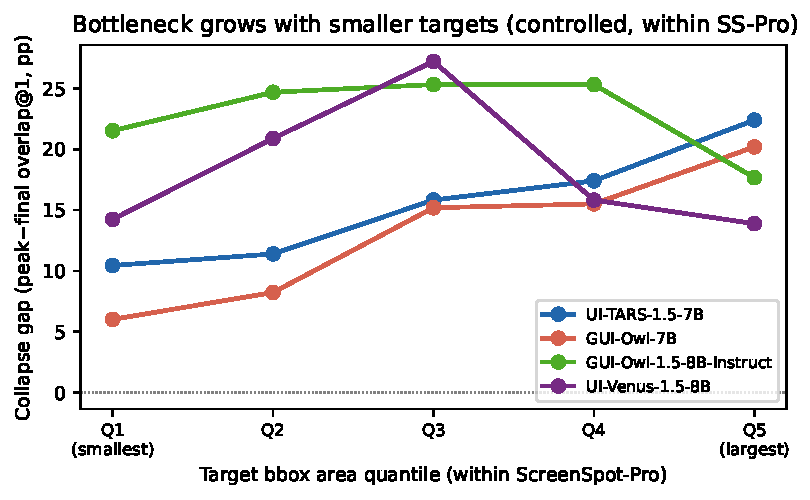
\includegraphics[width=0.92\columnwidth]{figs/fig_targetsize_gap.pdf}
\caption{\textbf{Collapse gap vs target-area quintile within ScreenSpot-Pro (hit@1).} The gap does not grow as targets shrink; the absolute final-layer accuracy (not the gap) is the cleaner severity measure and is worst on the smallest targets.}
\label{fig:targetsize_gap}
\end{figure}

\paragraph{Pre-scale visual-token norm census (4sok-Q4; cf.\ Vision Transformers Need Registers).}
Figure~\ref{fig:norm_census} measures the $\ell_2$-norm of the visual-patch
hidden states \emph{before} the RMSNorm pre-scale, i.e.\ the magnitude
information the pre-scale discards. The mean norm grows $\sim$3.4$\times$ from
layer 14 to layer 26 in both GUI-Owl-7B and UI-TARS-1.5-7B (Qwen2.5-VL),
directly confirming the depth-growth claim of \S\ref{sec:method:stage1}; a small
($\le 0.6\%$) but heavy-tailed set of outlier patches carries very high norm,
consistent with the attention-sink / register-token phenomenon---information
the pre-scale normalizes away but which a magnitude-aware variant could exploit.
\begin{figure}[t]
\centering
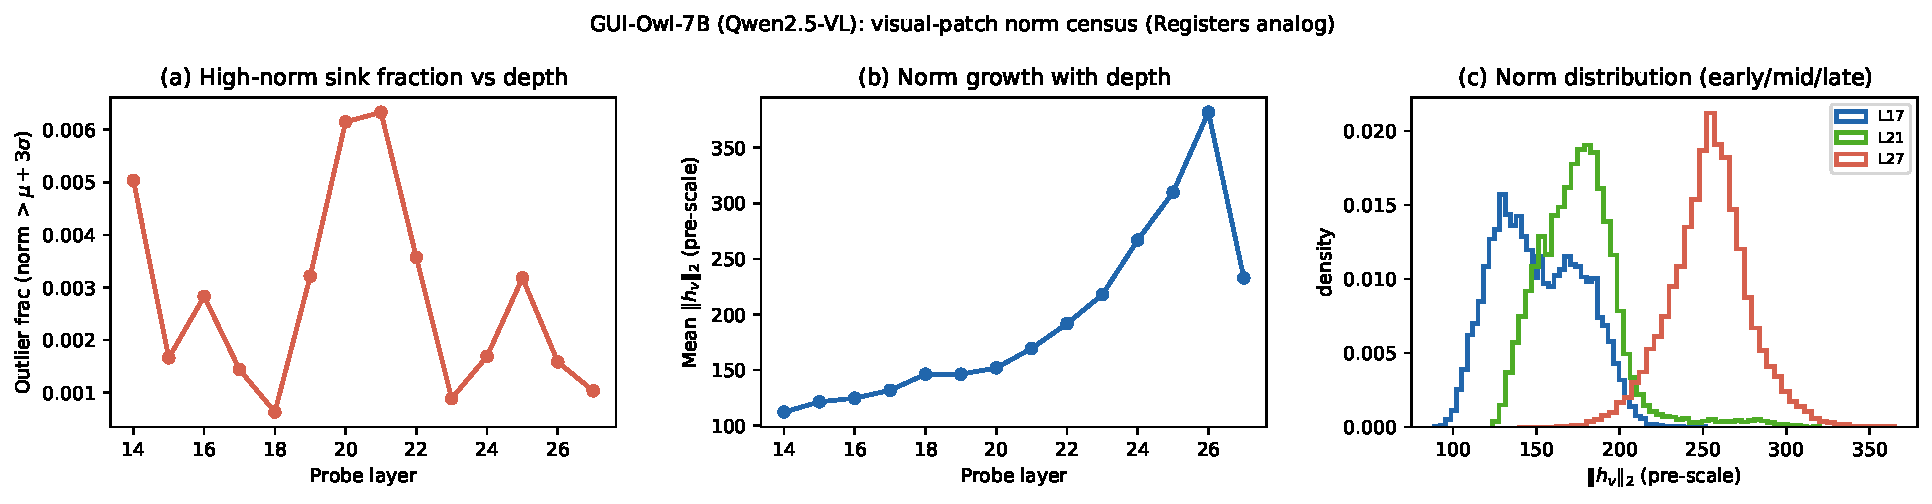
\includegraphics[width=0.95\columnwidth]{figs/fig_norm_census_guiowl7b.pdf}
\caption{\textbf{Pre-scale visual-patch norm census (GUI-Owl-7B, $n{=}100$).} (a) high-norm sink fraction vs depth; (b) mean $\|h_v\|_2$ grows $\sim$3.4$\times$ across depth; (c) norm distribution at early/mid/late layers (heavy-tailed).}
\label{fig:norm_census}
\end{figure}